\documentclass[utf8,a4paper]{ctexart}
\usepackage{float}
\usepackage{graphicx}
\usepackage{tocbibind}
\usepackage{appendix}
\usepackage{color}
\usepackage[format=hang,labelfont=bf]{caption}
\usepackage{geometry}
\usepackage{lastpage}
\usepackage{amsmath}
\usepackage{fancyhdr}
\pagestyle{fancy}
\lhead{
\includegraphics[scale=.8]{./img/logo.png}}
\rhead{\small\heiti 基于图像分割与模板匹配的车牌识别算法}
\cfoot{第 \thepage 页,共 \pageref{LastPage} 页}
\setlength{\headsep}{15mm}

\usepackage{listings}
\lstset{
    language=MATLAB,
    basicstyle=\ttfamily\small,
    aboveskip={1.0\baselineskip},
    belowskip={1.0\baselineskip},
    columns=fixed,
    extendedchars=true,
    breaklines=true,
    tabsize=4,
    prebreak=\raisebox{0ex}[0ex][0ex]{\ensuremath{\hookleftarrow}},
    frame=lines,
    showtabs=false,
    showspaces=false,
    showstringspaces=false,
    keywordstyle=\color[rgb]{0.627,0.126,0.941},
    commentstyle=\color[rgb]{0.133,0.545,0.133},
    stringstyle=\color[rgb]{01,0,0},
    numbers=left,
    numberstyle=\small,
    stepnumber=1,
    numbersep=10pt,
    captionpos=t,
    escapeinside={\%*}{*)}
}

\usepackage{listings}

\newtheorem{ass}{假设}

\begin{document}

\begin{titlepage}

    \begin{center}

        
\includegraphics[width=.9\textwidth]{./img/titlepage1.png}\\[.5cm]

        \textbf{\large SHANGHAI JIAO TONG UNIVERSITY}\\[.5cm]

        \textbf{\kaishu \huge 计算机视觉课程报告}\\[.5cm]

        
\includegraphics[width=.2\textwidth]{./img/titlepage2.png}\\[1.5cm]

        \begin{minipage}{0.23\textwidth}
            \begin{flushright} \large
                \textbf{\heiti 题目:}
            \end{flushright}
        \end{minipage}
        \begin{minipage}{0.67\textwidth}
            \begin{flushleft} \large
                \textbf{\heiti 基于图像分割与模板匹配的车牌识别算法}
            \end{flushleft}
        \end{minipage}\\[.5cm]

        \begin{minipage}{0.23\textwidth}
            \begin{flushright} \large
                \textbf{\heiti 评分:}
            \end{flushright}
        \end{minipage}
        \begin{minipage}{0.67\textwidth}
            \begin{flushleft} \large
                \textbf{\heiti }
            \end{flushleft}
        \end{minipage}\\[1.5cm]

        \begin{minipage}{0.2\textwidth}
            \begin{flushright} \large\kaishu
                学生姓名: \\
                学生学号: \\
                专\qquad 业: \\
                学院(系): \\
            \end{flushright}
        \end{minipage}
        \begin{minipage}{0.4\textwidth}
            \begin{flushleft} \large\kaishu
                \centering 郑宇森\\
                520021911173\\
                信息安全\\
                电子信息与电气工程学院
            \end{flushleft}
        \end{minipage}
        \vfill
        {\large \today}

    \end{center}

\end{titlepage}

\tableofcontents

\newpage

\section{绪论}
随着日常生活中汽车的使用量迅速增加,车牌识别愈发成为一种非常重要的技术手段,在违章拍照、智慧交通、车辆管理等领域有着广泛的应用。
同时,随着OCR、深度学习等新技术的迅猛发展,车牌识别算法也在更新迭代,许多准确高效的车牌识别算法不断涌现。
而本文作为一篇课程论文,将介绍一种基于图像分割与模板匹配的车牌识别算法,通过形态学处理、像素阈值分割等技术实现对目标车牌的识别。
\textbf{使用这一算法对提供的样例车牌进行识别,可以得到识别的准确率为$100\%$(识别结果见附录)},这证明了该算法的精确度和可靠性。
同时,笔者也筛选了一些其他已经预定位的车牌进行识别,发现准确度仍非常高,这证明了\textbf{字符分割与识别算法的泛化性很强}。
然而,由于形态学处理及色彩空间分割中使用的参数与具体图像环境有关,这使得\textbf{车牌定位算法的精确度与可靠性都有一定的局限性}。
最后,笔者\textbf{使用MATLAB程序实现了所有的算法流程,并封装成了一些简单的函数,可以在MATLAB环境中进行调试(程序见支撑文件)}。

\section{模型假设和符号说明}
\subsection{模型假设}
\begin{ass}
    假设识别的目标车牌为国内的普通汽车与新能源汽车,即车牌为蓝底白字或绿底黑字。由于日常生活中接触到的汽车主要为这两类,因此这一假设是具有普遍性的。
\end{ass}

\begin{ass}
    假设车牌为有规则长宽比的矩形区域。车牌字符为中文、英文、数字的有限集合,即使用模板匹配可以完全识别这些内容。
\end{ass}

\begin{ass}
    假设识别的车牌图像没有被污染,且没有模糊、毛刺、毛玻璃等现象。且图像中的车牌区域不出现强烈扭曲变形情况。
\end{ass}

\subsection{符号说明}

\begin{table}[H]
    \centering
    \caption{符号说明}
    \begin{tabular}{cc}
        \hline
        符号           & 解释                          \\
        \hline
        $P$            & $s\times t$的矫正后车牌区域图像矩阵                        \\
        $X_c$   & 备择区域(潜在字符区域横坐标)向量                                                 \\
        ${\mathrm d} X_c$ & 前向差分向量                                                 \\
        $A$ & $m \times n$单字符区域图像矩阵                                                 \\
        $T$ & 整形后$m\times n$模板图像矩阵                                                \\
        $|d|$ & 两幅图像的欧几里得距离                                                 \\
        \hline
    \end{tabular}
    \label{tab:my_label}
\end{table}

\section{算法结构}
本文介绍的图像分割与模板匹配的车牌识别算法由\textbf{车牌定位、字符分割与字符识别}三个模块组成。

对于输入图像,首先计算兴趣域的掩膜,初步确定车牌的位置,然后进行形态学运算,通过膨胀与腐蚀获取车的边界点。进而通过四点透视法获取矫正后的车牌图像。

在字符分割部分,我们先获取图像二值化阈值,对图像二值化处理。而后判断白色像素占比,判断是否要进行反色处理(针对新能源汽车的车牌)。再统计行、列的白色像素点数目,通过差分运算获取字符的起始与终止位置,进而完成分割。

在字符识别部分,我们计算每个字符与模板字符库中字符的欧几里得距离。同时为了提高精度,我们还求了每组字符的平均值。最终我们认为平均距离最小的字符为识别出的字符。

流程图如图~\ref{fig:plate_recognition}所示。

\begin{figure}[h]
    \centering
    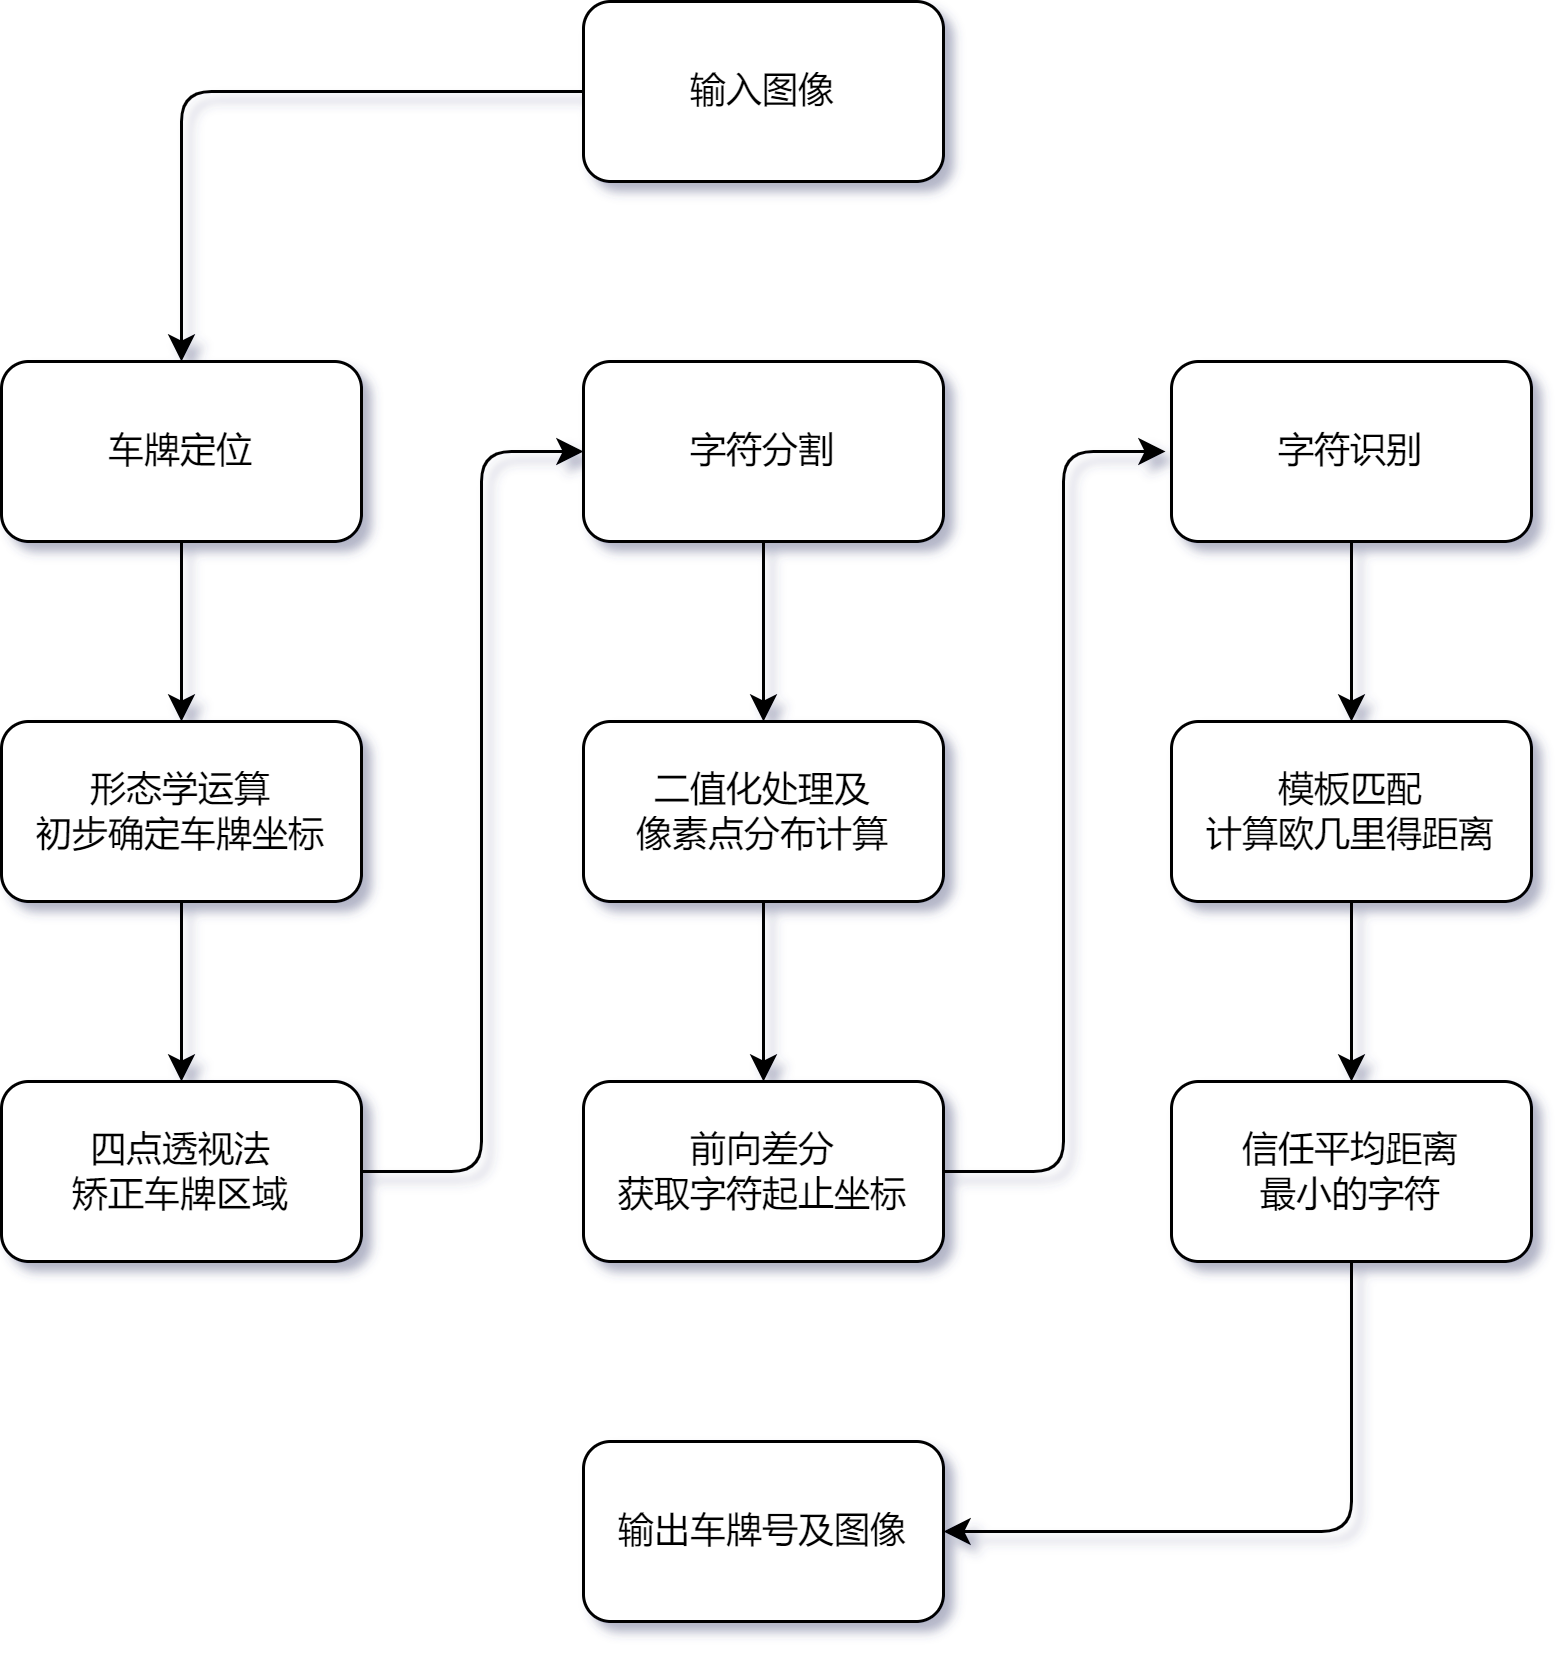
\includegraphics[width=0.6\textwidth]{./img/pic.png}
    \caption{算法流程图}
    \label{fig:plate_recognition}
\end{figure}

\section{车牌定位}
\subsection{兴趣域掩膜}
由于我们已知车牌颜色的一些先验知识,我们可以对输入图像的色彩空间进行分割,将多通道图像的色彩空间分割为单独的R、G、B通道。
进而我们根据待识别图像的色彩特征,对各个通道选取合适的阈值,并信任阈值内的区域为可能存在车牌的区域。
根据计算得到的结果,我们得到该区域的掩膜,如图~\ref{fig:mask}所示。

\subsection{形态学运算获取车牌边界}
由图像可知,掩膜周围存在不平滑的噪点,且掩膜中的字体呈现镂空效果,这均不利于我们确定车牌的边界。

因此,我们一方面通过形态学膨胀运算,使车牌区域更加明显可见并填充车牌中的字体区域;
一方面通过形态学腐蚀运算,去除了孤立点和小对象,因此只剩下重要的车牌区域。处理结果如图~\ref{fig:morphology}所示。

\begin{minipage}{0.44\linewidth}
    \begin{figure}[H]
        \center
        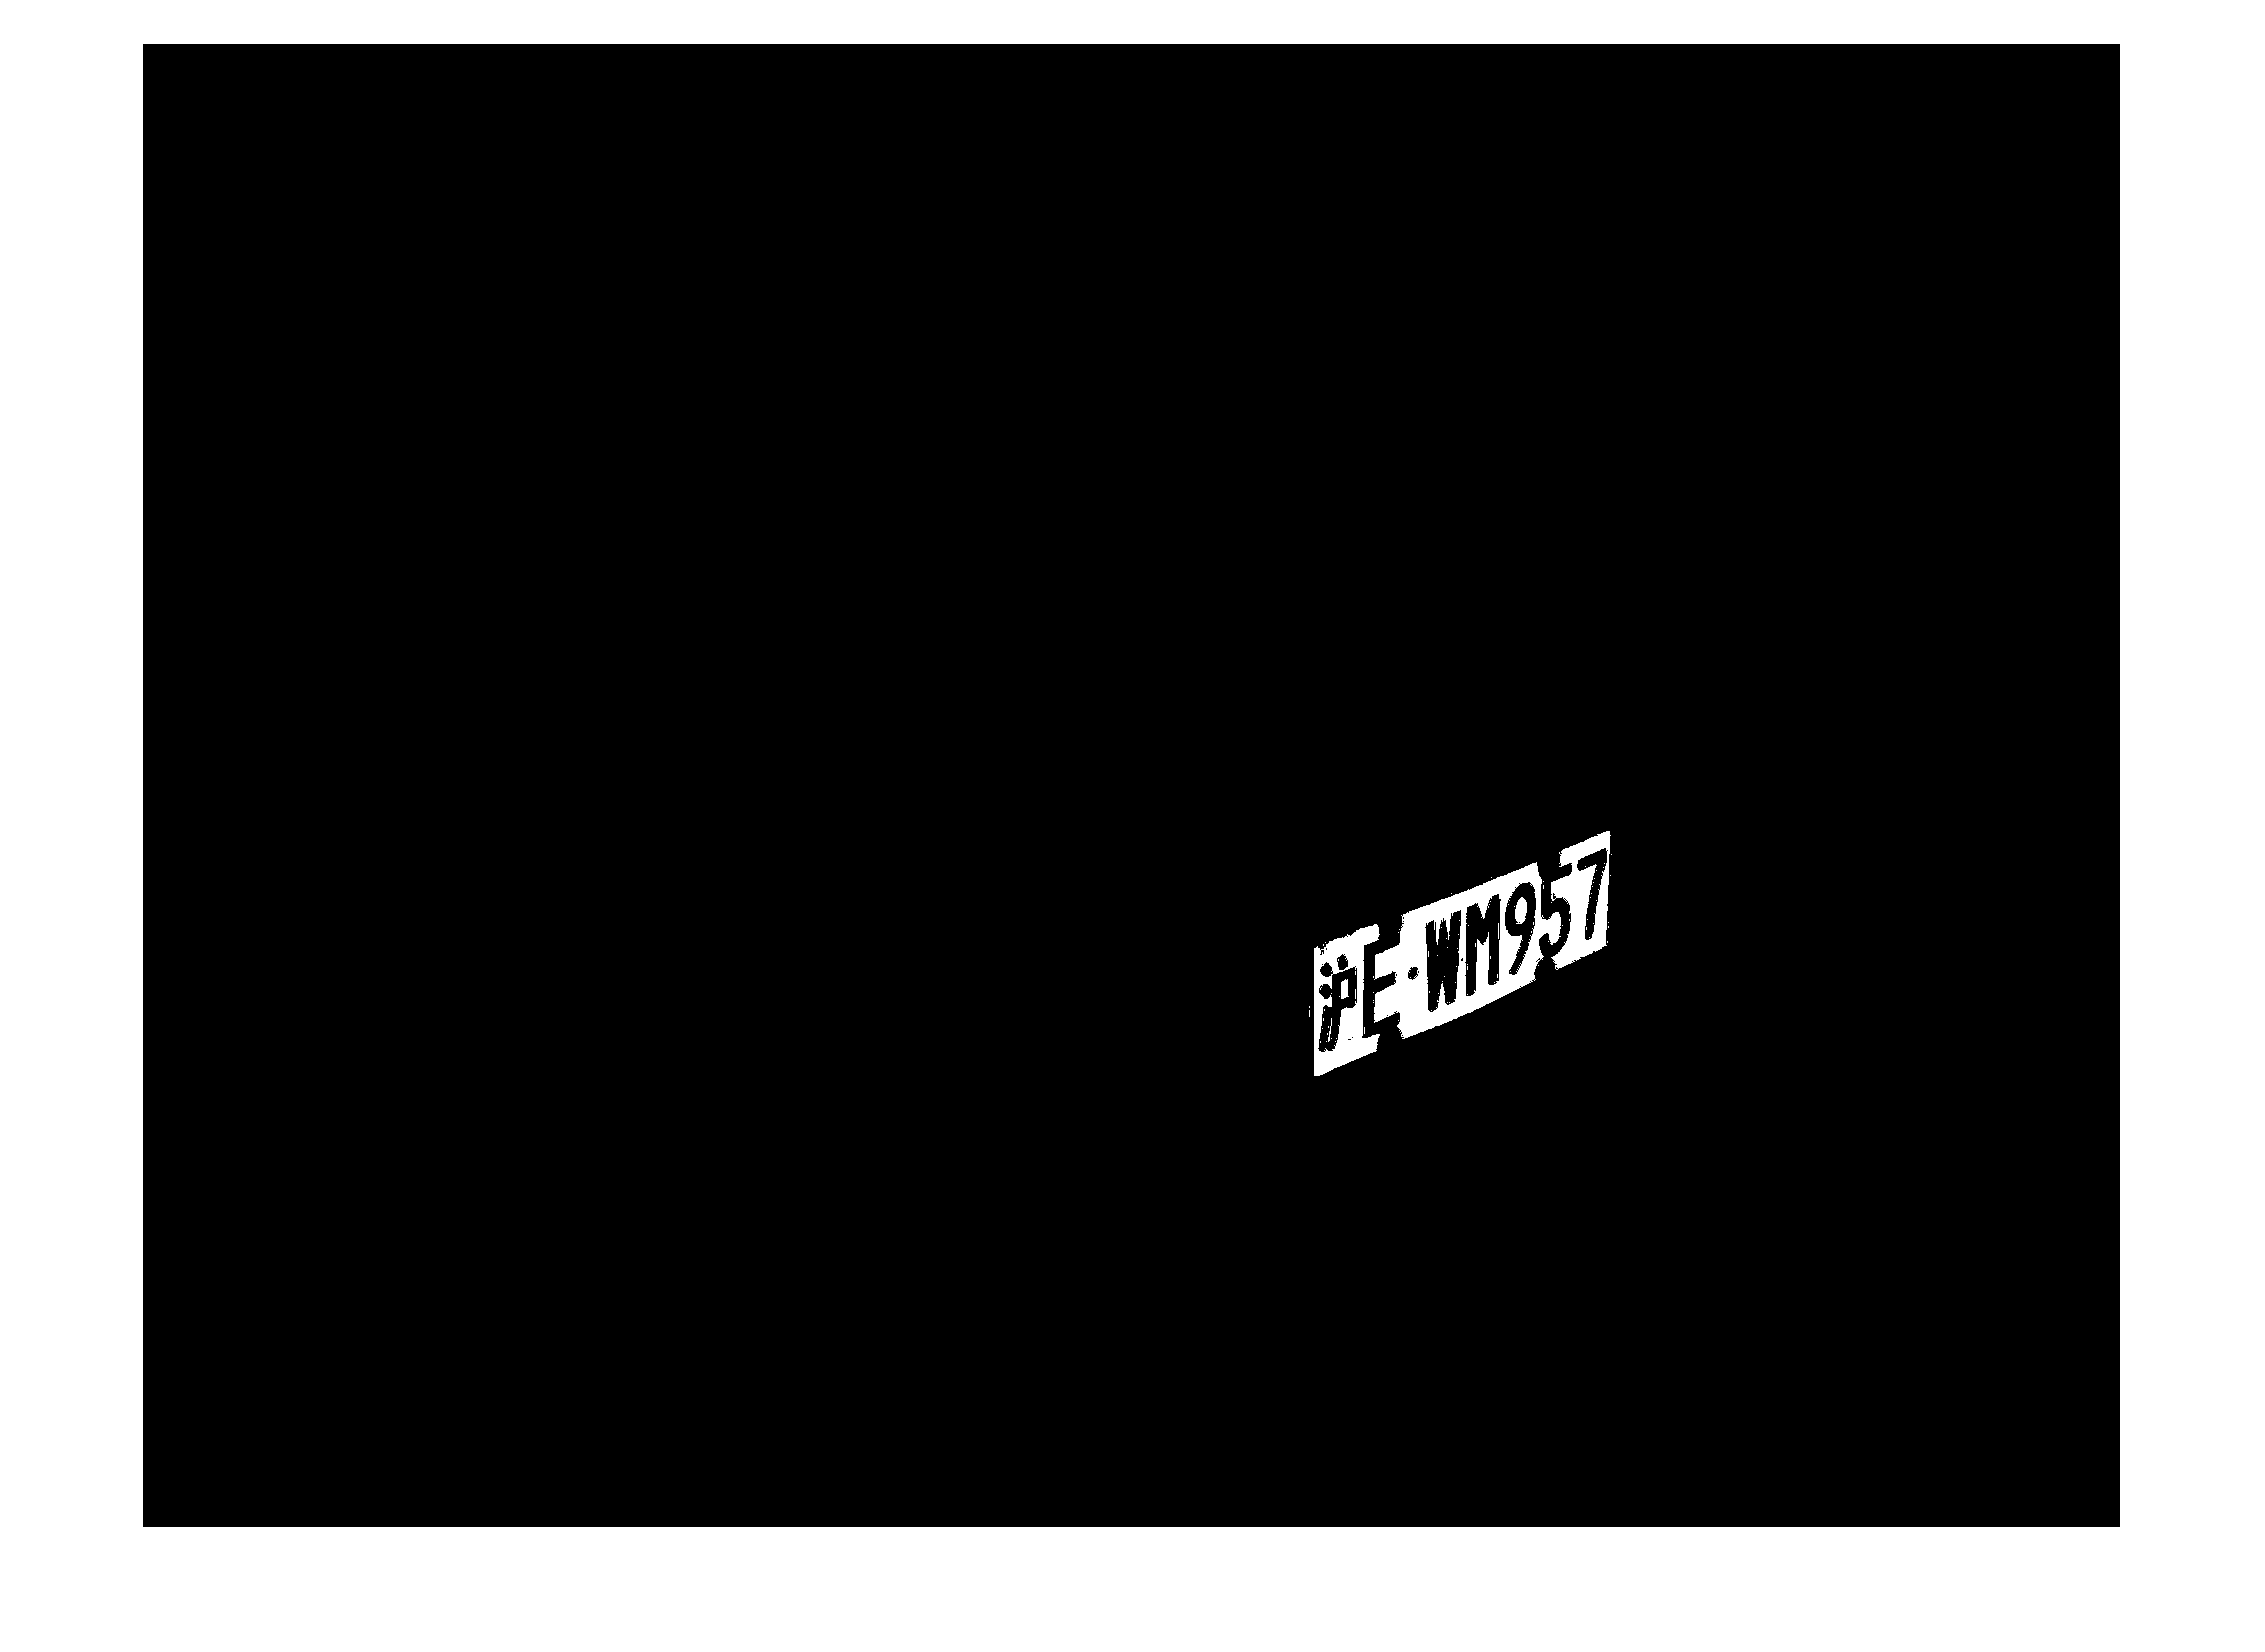
\includegraphics[width=\linewidth]{./img/difficult/掩膜.png}
        \caption{获取掩膜}
        \label{fig:mask}
    \end{figure}
\end{minipage}
\hfill
\begin{minipage}{0.44\linewidth}
    \begin{figure}[H]
        \center
        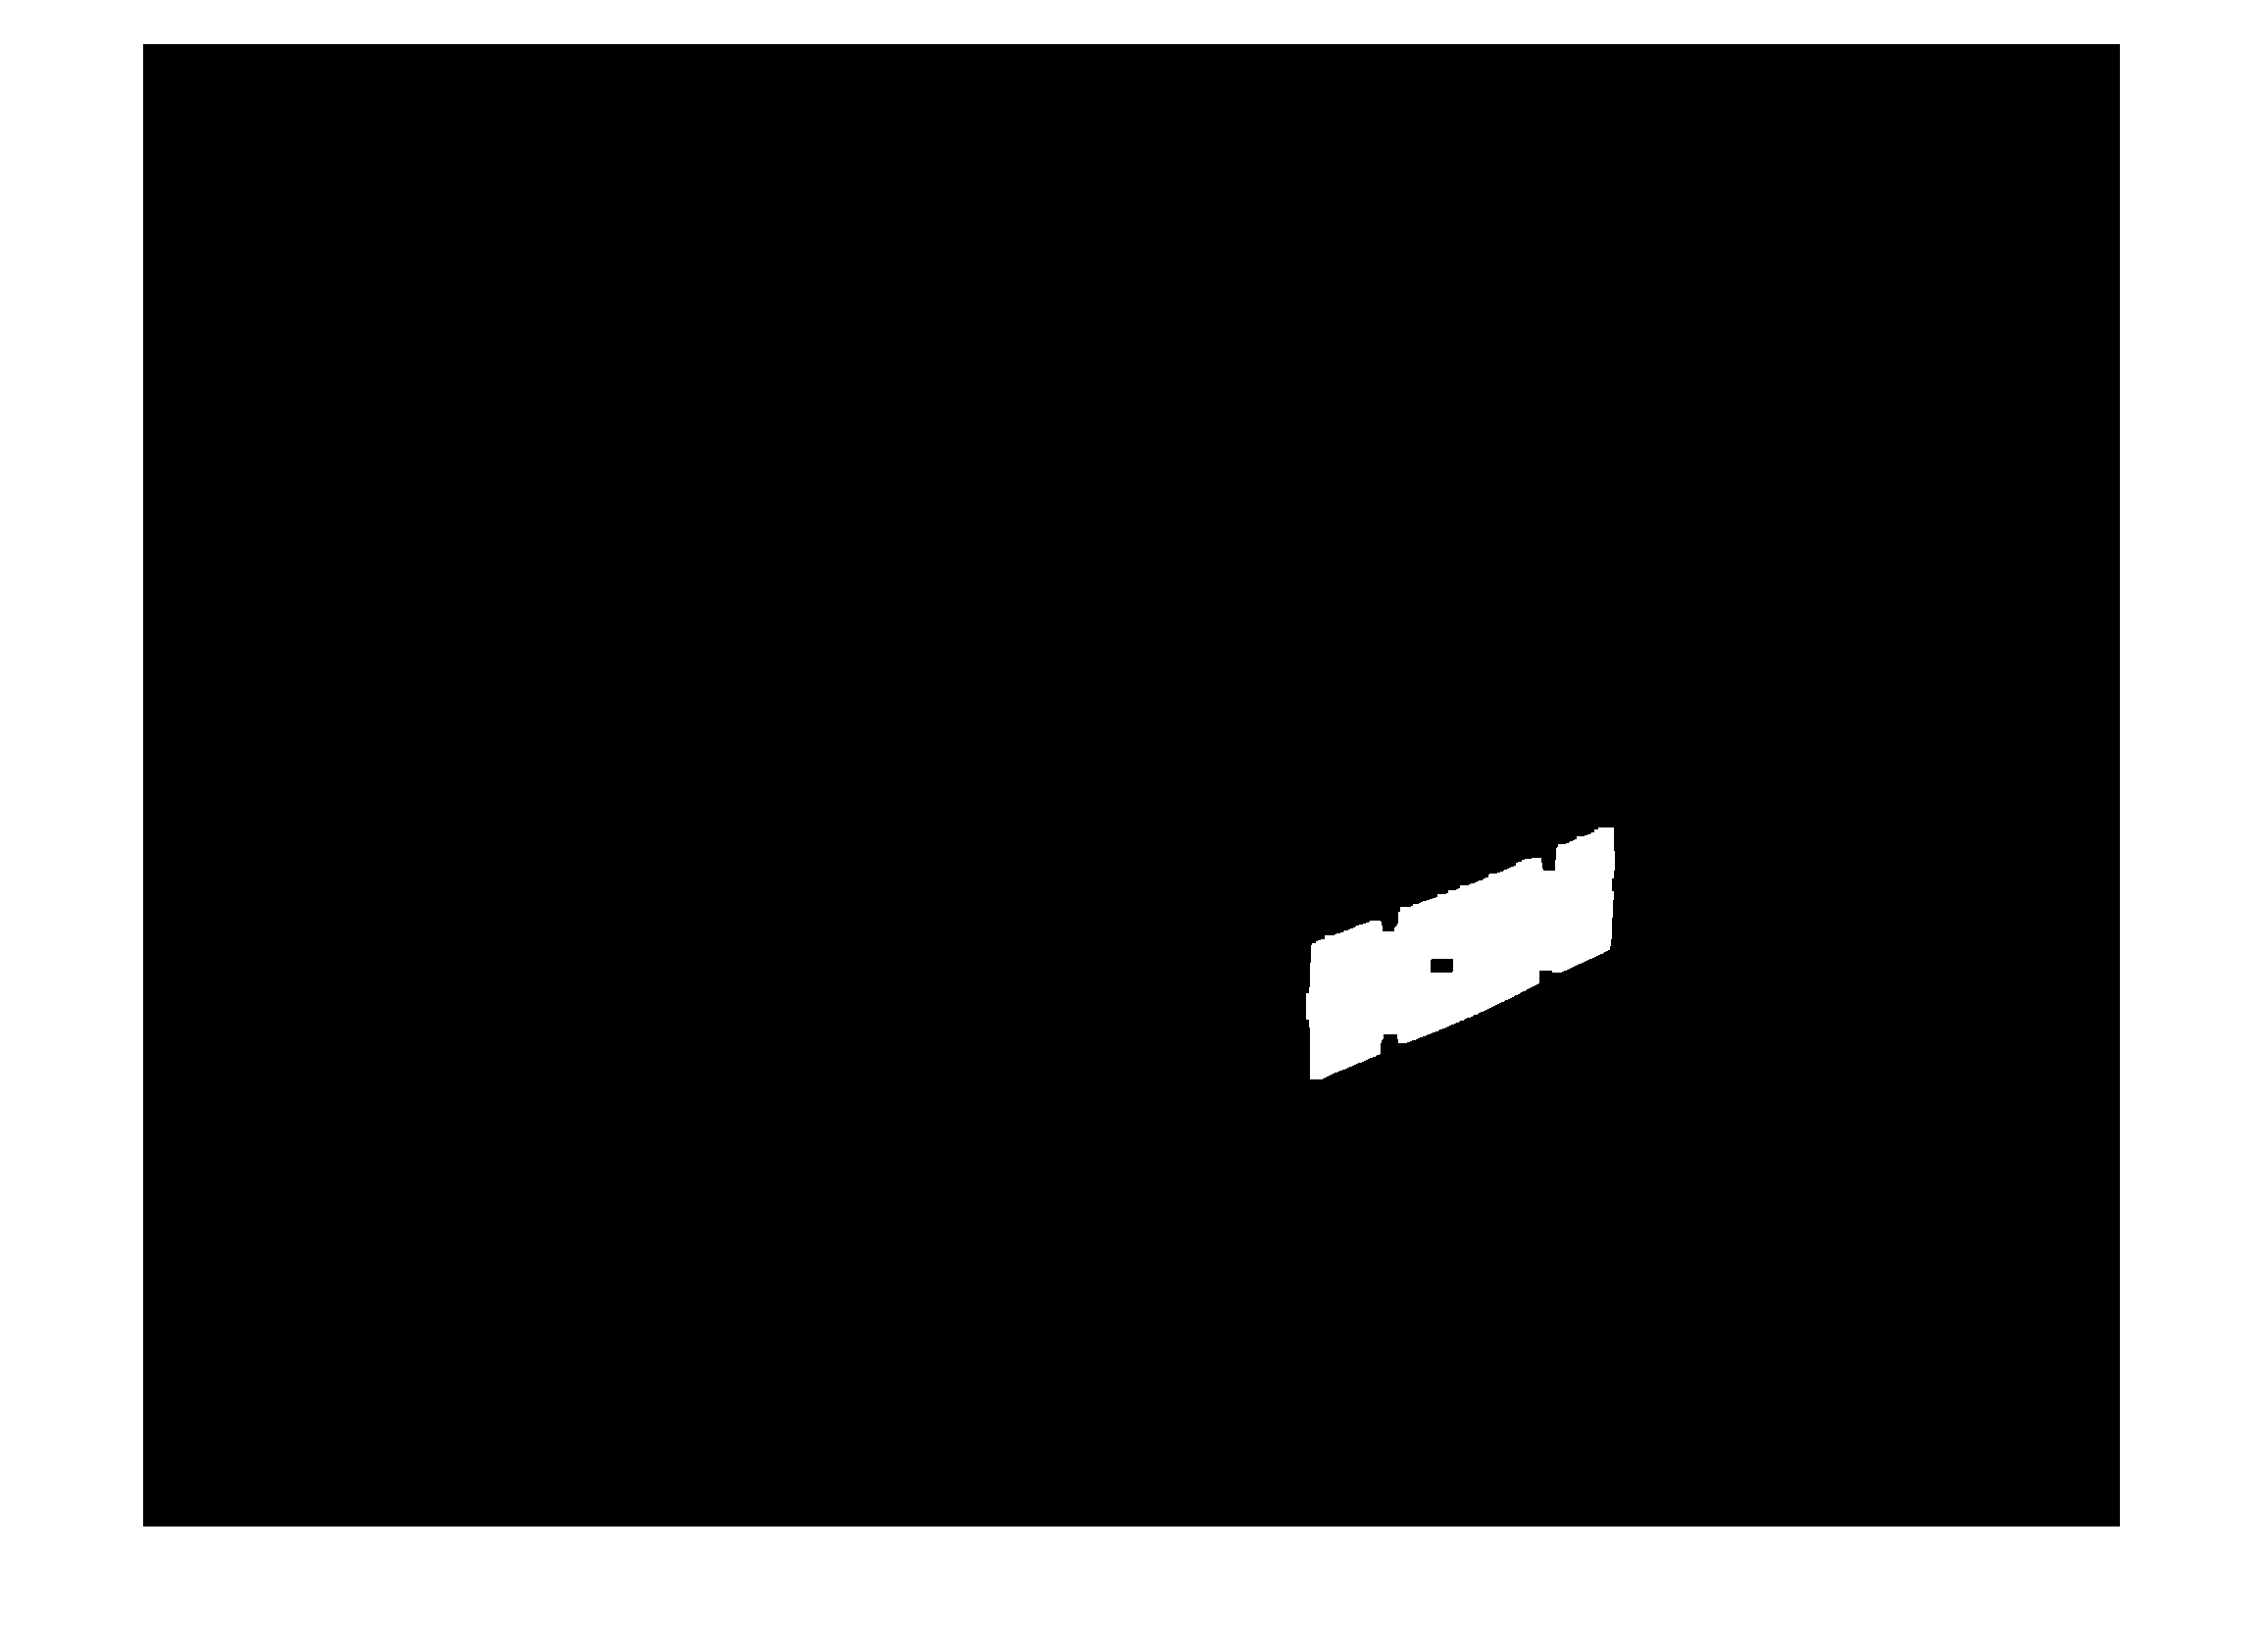
\includegraphics[width=\linewidth]{./img/difficult/形态学运算.png}
        \caption{形态学运算获取边界}
        \label{fig:morphology}
    \end{figure}
\end{minipage}
\par

\subsection{四点法倾斜矫正}
由于部分样例图像中车牌呈倾斜状,因此我们需要对图像进行透视变换矫正,从而得到规则的车牌区域。
我们首先计算图像的四个角点,作为原图像标定点。
进而选取合适的微小变化量,微调后得到目标矩形(规则地车牌区域)的四个角点。
通过标定点与目标点,我们可以计算出图像的透视变换矩阵,对图像进行透视变换。
最终得到透视矫正后的车牌区域。矫正流程如图~\ref{fig:perspective},图~\ref{fig:crop}与图~\ref{fig:correct}所示。

\begin{figure}[H]
    \center
    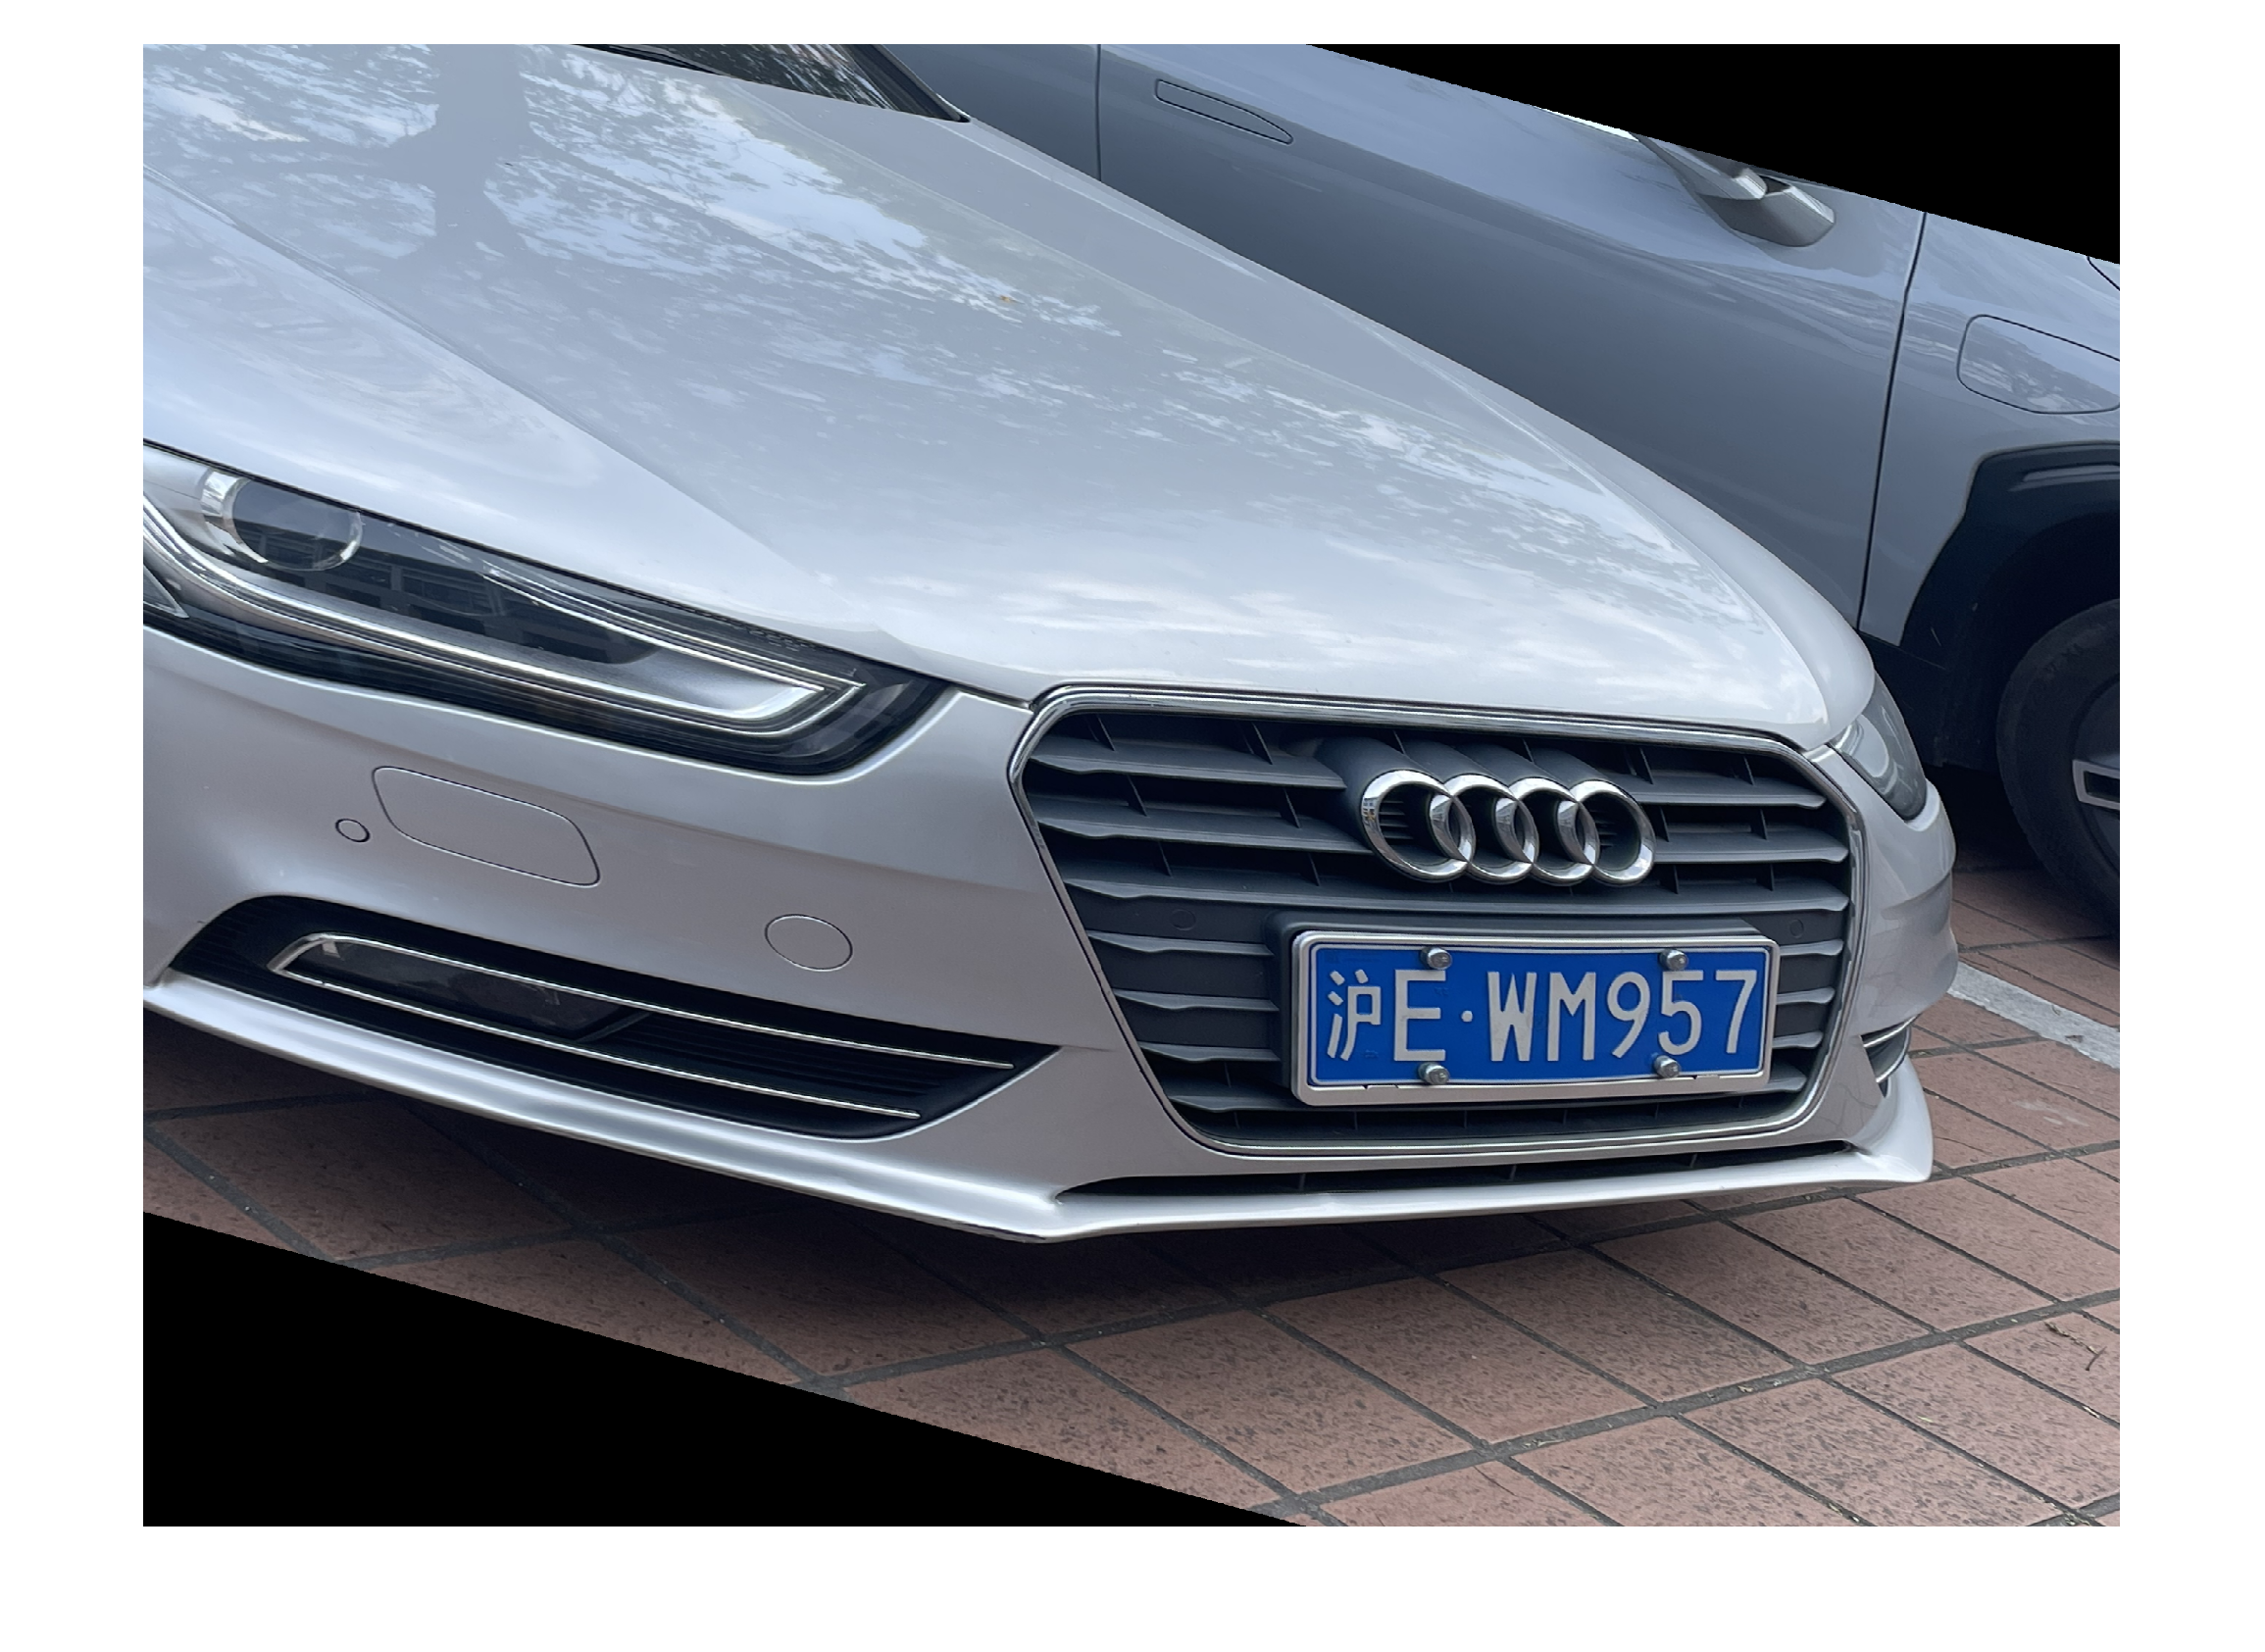
\includegraphics[width=.6\textwidth]{./img/difficult/矫正.png}
    \caption{矫正后图像}
    \label{fig:perspective}
\end{figure}

\begin{minipage}{0.44\linewidth}
    \begin{figure}[H]
        \center
        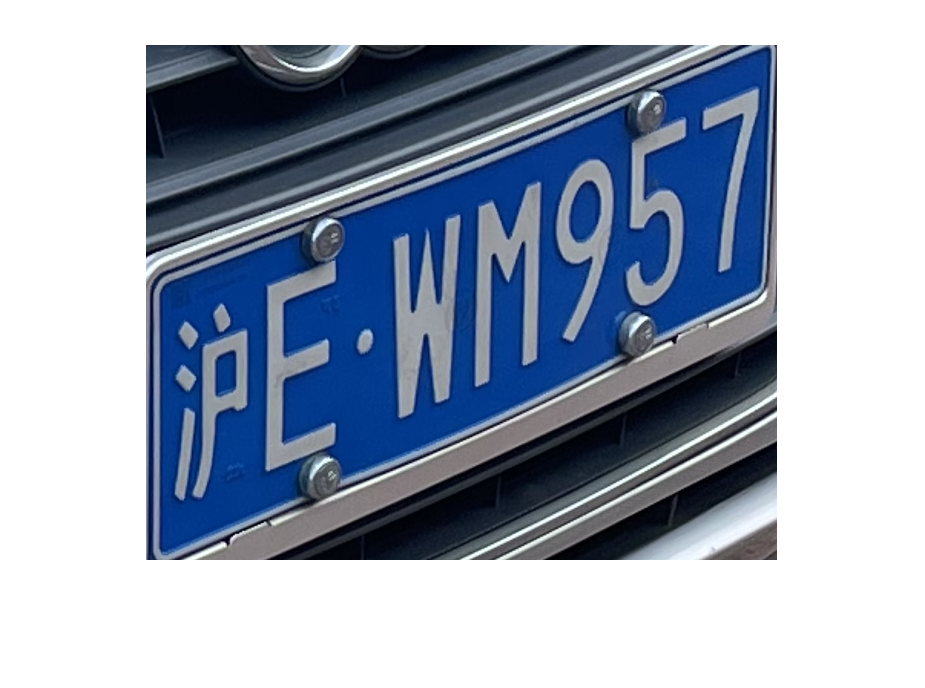
\includegraphics[width=\linewidth]{./img/difficult/定位.png}
        \caption{截取车牌区域}
        \label{fig:crop}
    \end{figure}
\end{minipage}
\hfill
\begin{minipage}{0.44\linewidth}
    \begin{figure}[H]
        \center
        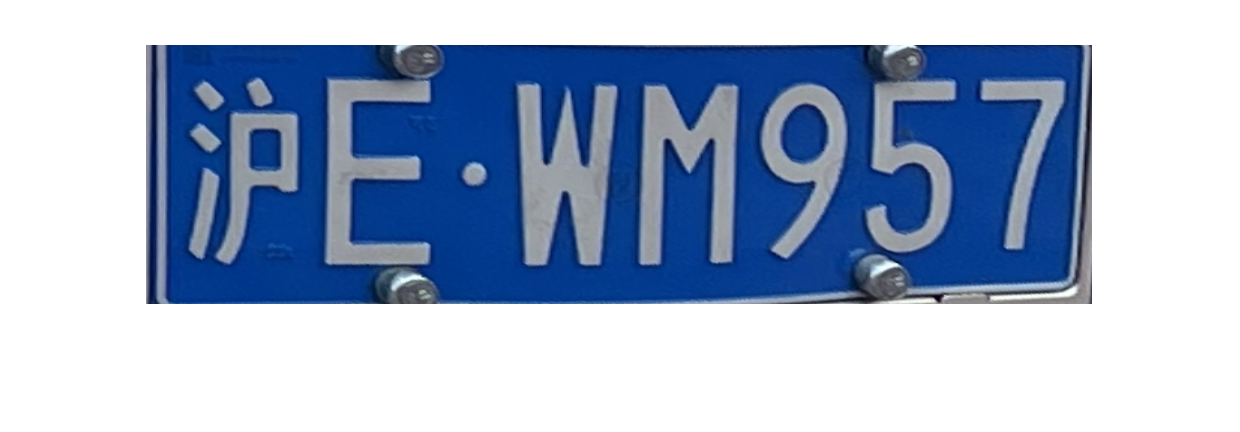
\includegraphics[width=\linewidth]{./img/difficult/截取.png}
        \caption{矫正后的车牌区域}
        \label{fig:correct}
    \end{figure}
\end{minipage}
\par

\section{字符分割}
\subsection{图像预处理}
为了防止图像中的噪点影响分割过程,我们首先对已经定位好的车牌图像进行高斯模糊,并绘制得到灰度阈值直方图如图~\ref{fig:hist}。

\begin{figure}[h]
    \centering
    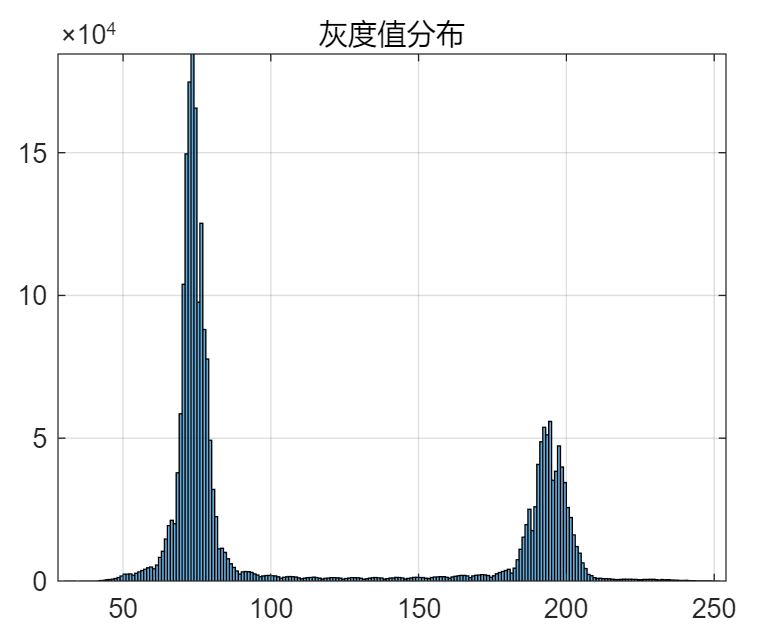
\includegraphics[width=0.6\textwidth]{./img/easy/灰度阈值可视化.png}
    \caption{灰度直方图}
    \label{fig:hist}
\end{figure}

可以看到,直方图有明显的双峰特征。于是我们可以选取一个阈值,将图像二值化,结果如图~\ref{fig:preprocess}。

\begin{figure}[h]
    \centering
    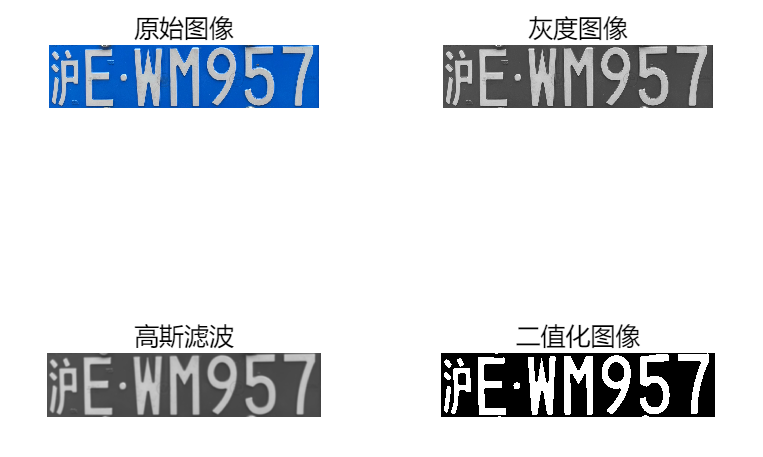
\includegraphics[width=0.8\textwidth]{./img/easy/处理效果可视化.png}
    \caption{图像预处理}
    \label{fig:preprocess}
\end{figure}

普通汽车的车牌字体颜色比背景颜色浅,故普通汽车车牌经过二值化处理后,字体为白色,背景为黑色。
然而部分新能源汽车的车牌字体颜色深于背景颜色,为了统一封装后续处理过程,我们对其进行反色处理。
反色的判据为若白色像素点占比超出$50\%$,则认为需要反色。
另一项处理是在二值化后的车牌图像矩阵的左右两侧各增加一全为$0$的列,这是为了后续差分运算的方便,以免出现第一列无法计算前向差分的情况。

\subsection{直方图字符分割}
我们计算每列的白色像素点数目,得到白色像素点列累加直方图,将数值大于选取阈值的区域视为备择区域,效果如图~\ref{fig:pixel_count}。

备择区域向量$X_c$和前向差分向量${\mathrm d} X_c$的构造如下。

\begin{equation}
    X_c[i] =
    \begin{cases}
        0,\  \sum_{j=1}^tP <threshold \\
        1,\  \sum_{j=1}^tP \geq threshold
    \end{cases},\ \forall i=1,2,\cdots,s
\end{equation}

\begin{equation}
    {\mathrm d} X_c[i] = X_c[i]-X_c[i-1],\ \forall i=2,3,\cdots,s
\end{equation}

其中$P$为$s\times t$的车牌区域图像矩阵。

\begin{figure}[h]
    \centering
    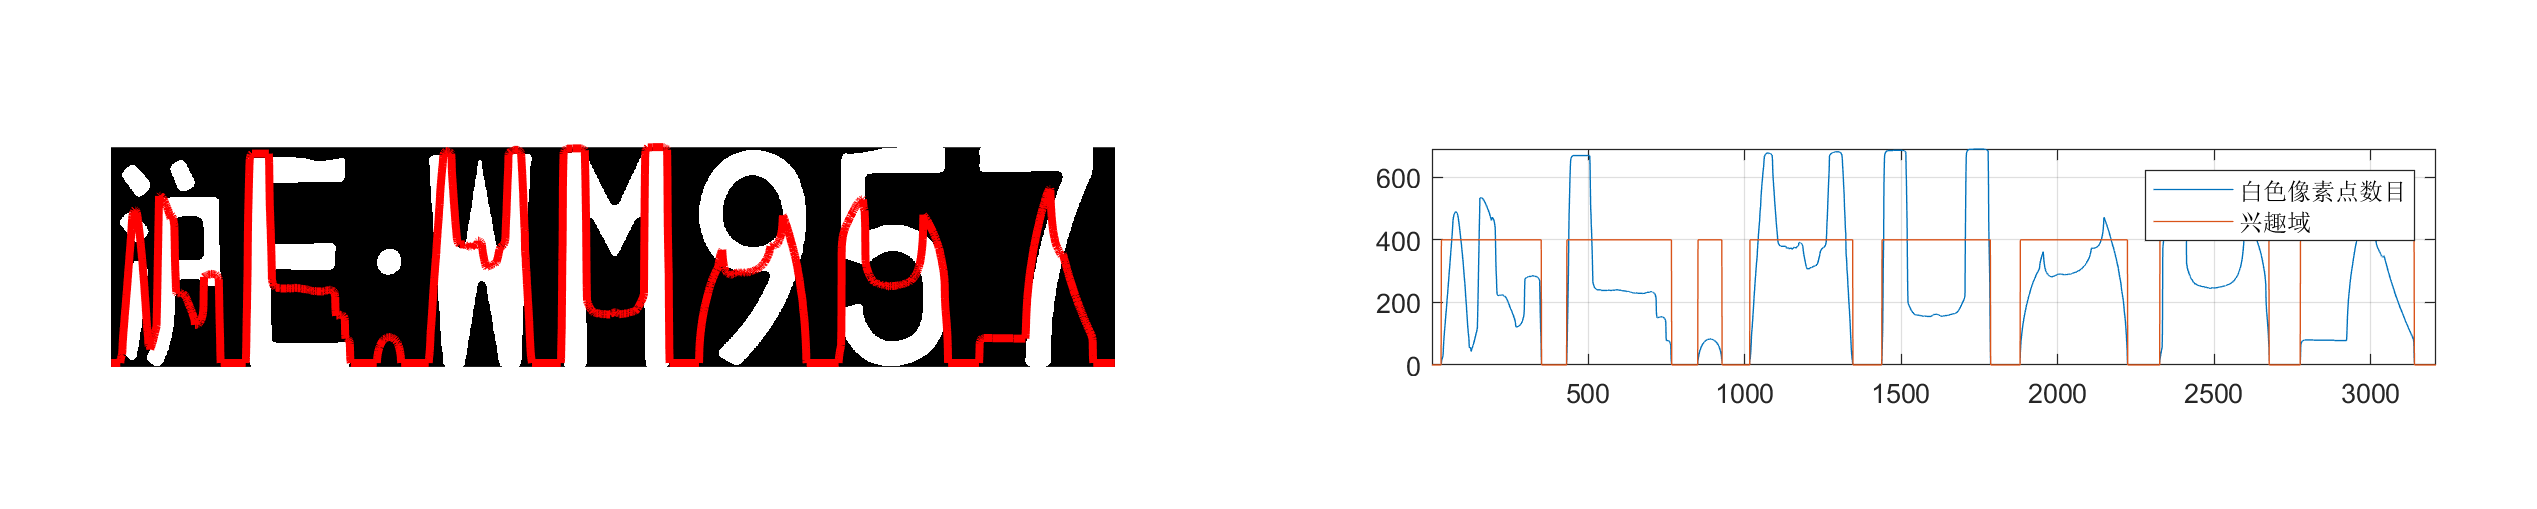
\includegraphics[width=0.8\textwidth]{./img/easy/双图.png}
    \caption{像素点统计}
    \label{fig:pixel_count}
\end{figure}

对备择区域做前向差分,即可得到阈值突变点的横坐标,这些横坐标即为车牌的潜在分割点。
每个上升沿和对应的下降沿内的区域为潜在的字符区域。

\subsection{矫正处理}
若直接认为上一步骤中得到的字符区域是单个字符,可能会出现分割了原子字符的情况,如将``沪''分割成``氵''和``户''两个字符。
因此我们需要对分割结果进行矫正处理。我们使用的方法是计算所有无字符的间隔区域长度,并计算得到平均值,
小于平均值的二分之一的间隔区域将被视作联通区域,该区域不被分割,从而保证字符的完整性。
此外,由于车牌中有分隔符``·'',有时还会出现尖锐的噪声区域,我们也需要对其进行处理。我们计算所有字符区域的长度,并计算得到平均值,
小于平均值的二分之一的字符区域将被视作分隔符或噪声区域,该区域被丢弃,从而保证字符的有效性。

最终差分与分割结果如图~\ref{fig:split_result}。

\begin{figure}[h]
    \centering
    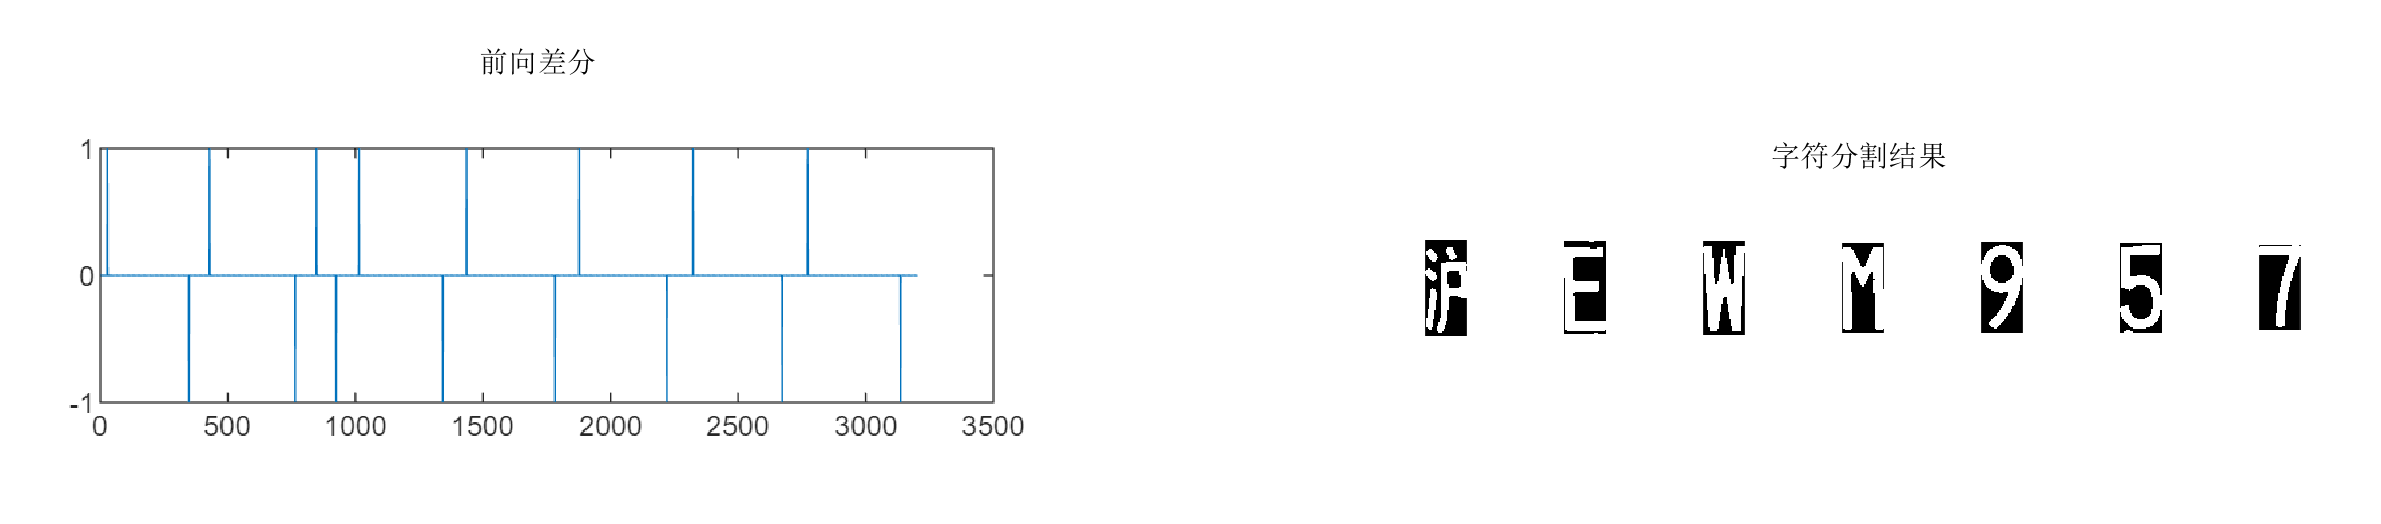
\includegraphics[width=0.8\textwidth]{./img/easy/双图2.png}
    \caption{差分及分割结果}
    \label{fig:split_result}
\end{figure}


\section{字符识别}
在字符识别阶段,我们使用模板字符库,为了提高匹配的精度和可信度,
每个模板字符均包含多张图片(如每个模板字符``沪''包含多张不同角度的``沪''字灰度图片)。
首先,我们将字符分割中得到的每个单字符区域进行模板匹配,其中模板字符需要放缩调整到单字符区域大小,以便后续运算。

进而,我们计算分割字符与每个整形后的模板字符的欧几里得距离,定义如下

\begin{equation}
    d^2=\sum_{i=1}^{m}\sum_{j=1}^n(A[i,j]-T[i,j])^2
\end{equation}

其中$|d|$为欧几里得距离,$A$为$m\times n$分割后待识别字符图像矩阵,$T$为模板字符图像矩阵。

我们计算待识别字符与每个模板字符库中所有字符图像的欧几里得距离的平均值,并信任平均值最小的识别结果。
以``沪''为例,识别效果如图~\ref{fig:template_match}。由图可见,对于正确匹配的模板字符,
待识别字符的欧几里得距离会显著低于非正确匹配的其他模板字符,因此这种方式具有较高的识别精度。

\begin{figure}[h]
    \centering
    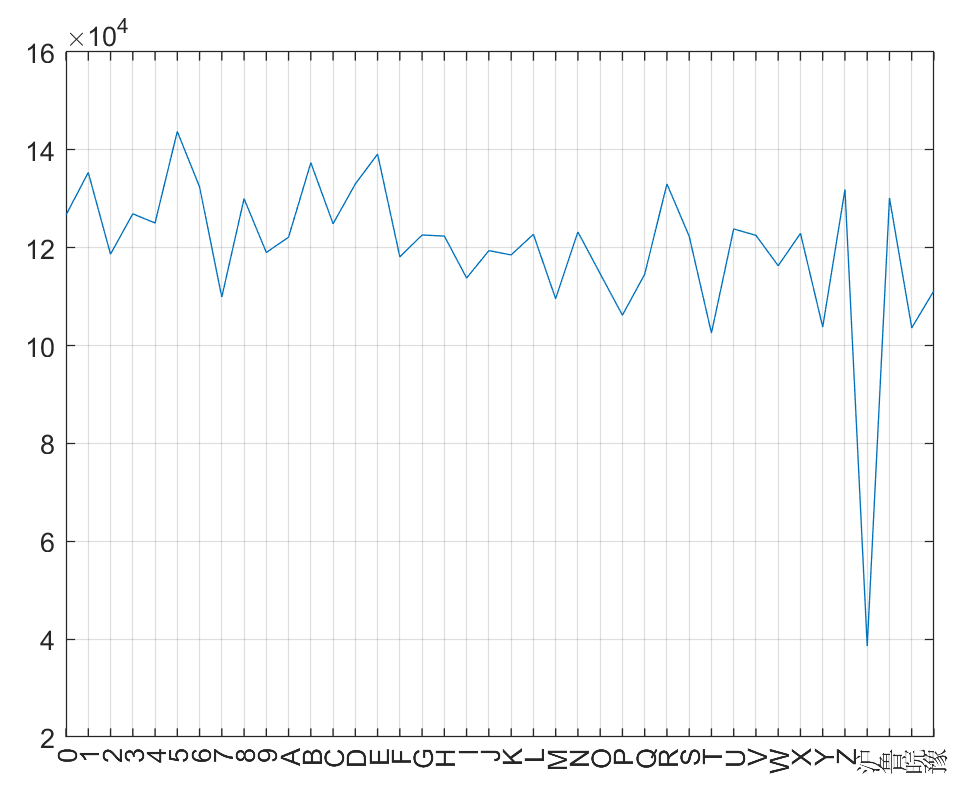
\includegraphics[width=0.6\textwidth]{./img/easy/识别效果可视化.png}
    \caption{模板匹配结果}
    \label{fig:template_match}
\end{figure}

\section{评价、总结与展望}
\subsection{评价}
回顾整个算法流程,\textbf{我们使用了一种非深度学习的传统视觉方法,准确完成了所有样例车牌的识别。
整个流程较好地体现了计算机视觉领域中敏锐高效地搜寻、提取、利用图像特征的思想。}
除准确度外,我们也可以提出其他评价标准,例如能否识别运动车辆的车牌,识别结果鲁棒性、识别速度的即时性等。
为此,我也寻找并筛选出一些预定位好的车牌图像,使用本文中的识别算法进行识别,结果仍然是鲁棒的。

\subsection{算法优点}
\begin{itemize}
    \item 本文使用的算法是一种非深度学习的方法,其算法结构简单,\textbf{可移植性强}。
    \item 本文中字符分割与模板匹配算法考虑了多种特殊情况(如不同车牌种类、分隔符处理、纠正原子字符分割等),并相应地做出了矫正处理,这使得算法具有\textbf{很强的泛化能力}。
    \item 字符分割算法中,笔者尝试了选取不同的白色像素点阈值,在正常范围内(阈值不过小),识别结果未受到干扰,这说明该阈值具有\textbf{较高的鲁棒性}。
\end{itemize}

\subsection{算法不足}
\begin{itemize}
    \item 车牌定位部分算法中,色彩空间的分割阈值与透视矫正的微小变量与具体图像有关,因此对于不同的输入图像,输出矫正图像的精度有较大的差异,需要人工调整阈值。
    \item 模板匹配中使用不同的模板对识别结果稍有影响,这或可以通过使用深度学习中CNN、RNN网络进行训练,为不同模板分配合适的权重来完善。
\end{itemize}

\section{谢辞}
作为一名本科二年级学生,由于没有接触过数字图像处理、机器学习等前置课程的学习,我在学习计算机视觉课程中遇到了许多挑战。
在此我要诚挚地感谢赵旭老师详细的讲解,让我在学习过程中有了更多的灵感,更深入的理解了计算机视觉的概念。
我也要感谢两位助教老师的耐心指导,帮助我解答了许多课程与作业中的困惑。

\newpage

\begin{appendices}
    \section*{\LARGE 附录}

    \section{识别结果}
    使用本文中提出的算法,车牌识别结果如下,其中\textbf{识别的车牌字符串作为输出图片的标题,在图片上方显示}。

    \centering{\textbf{命令行输出结果}}

    \begin{figure}[H]
        \center
        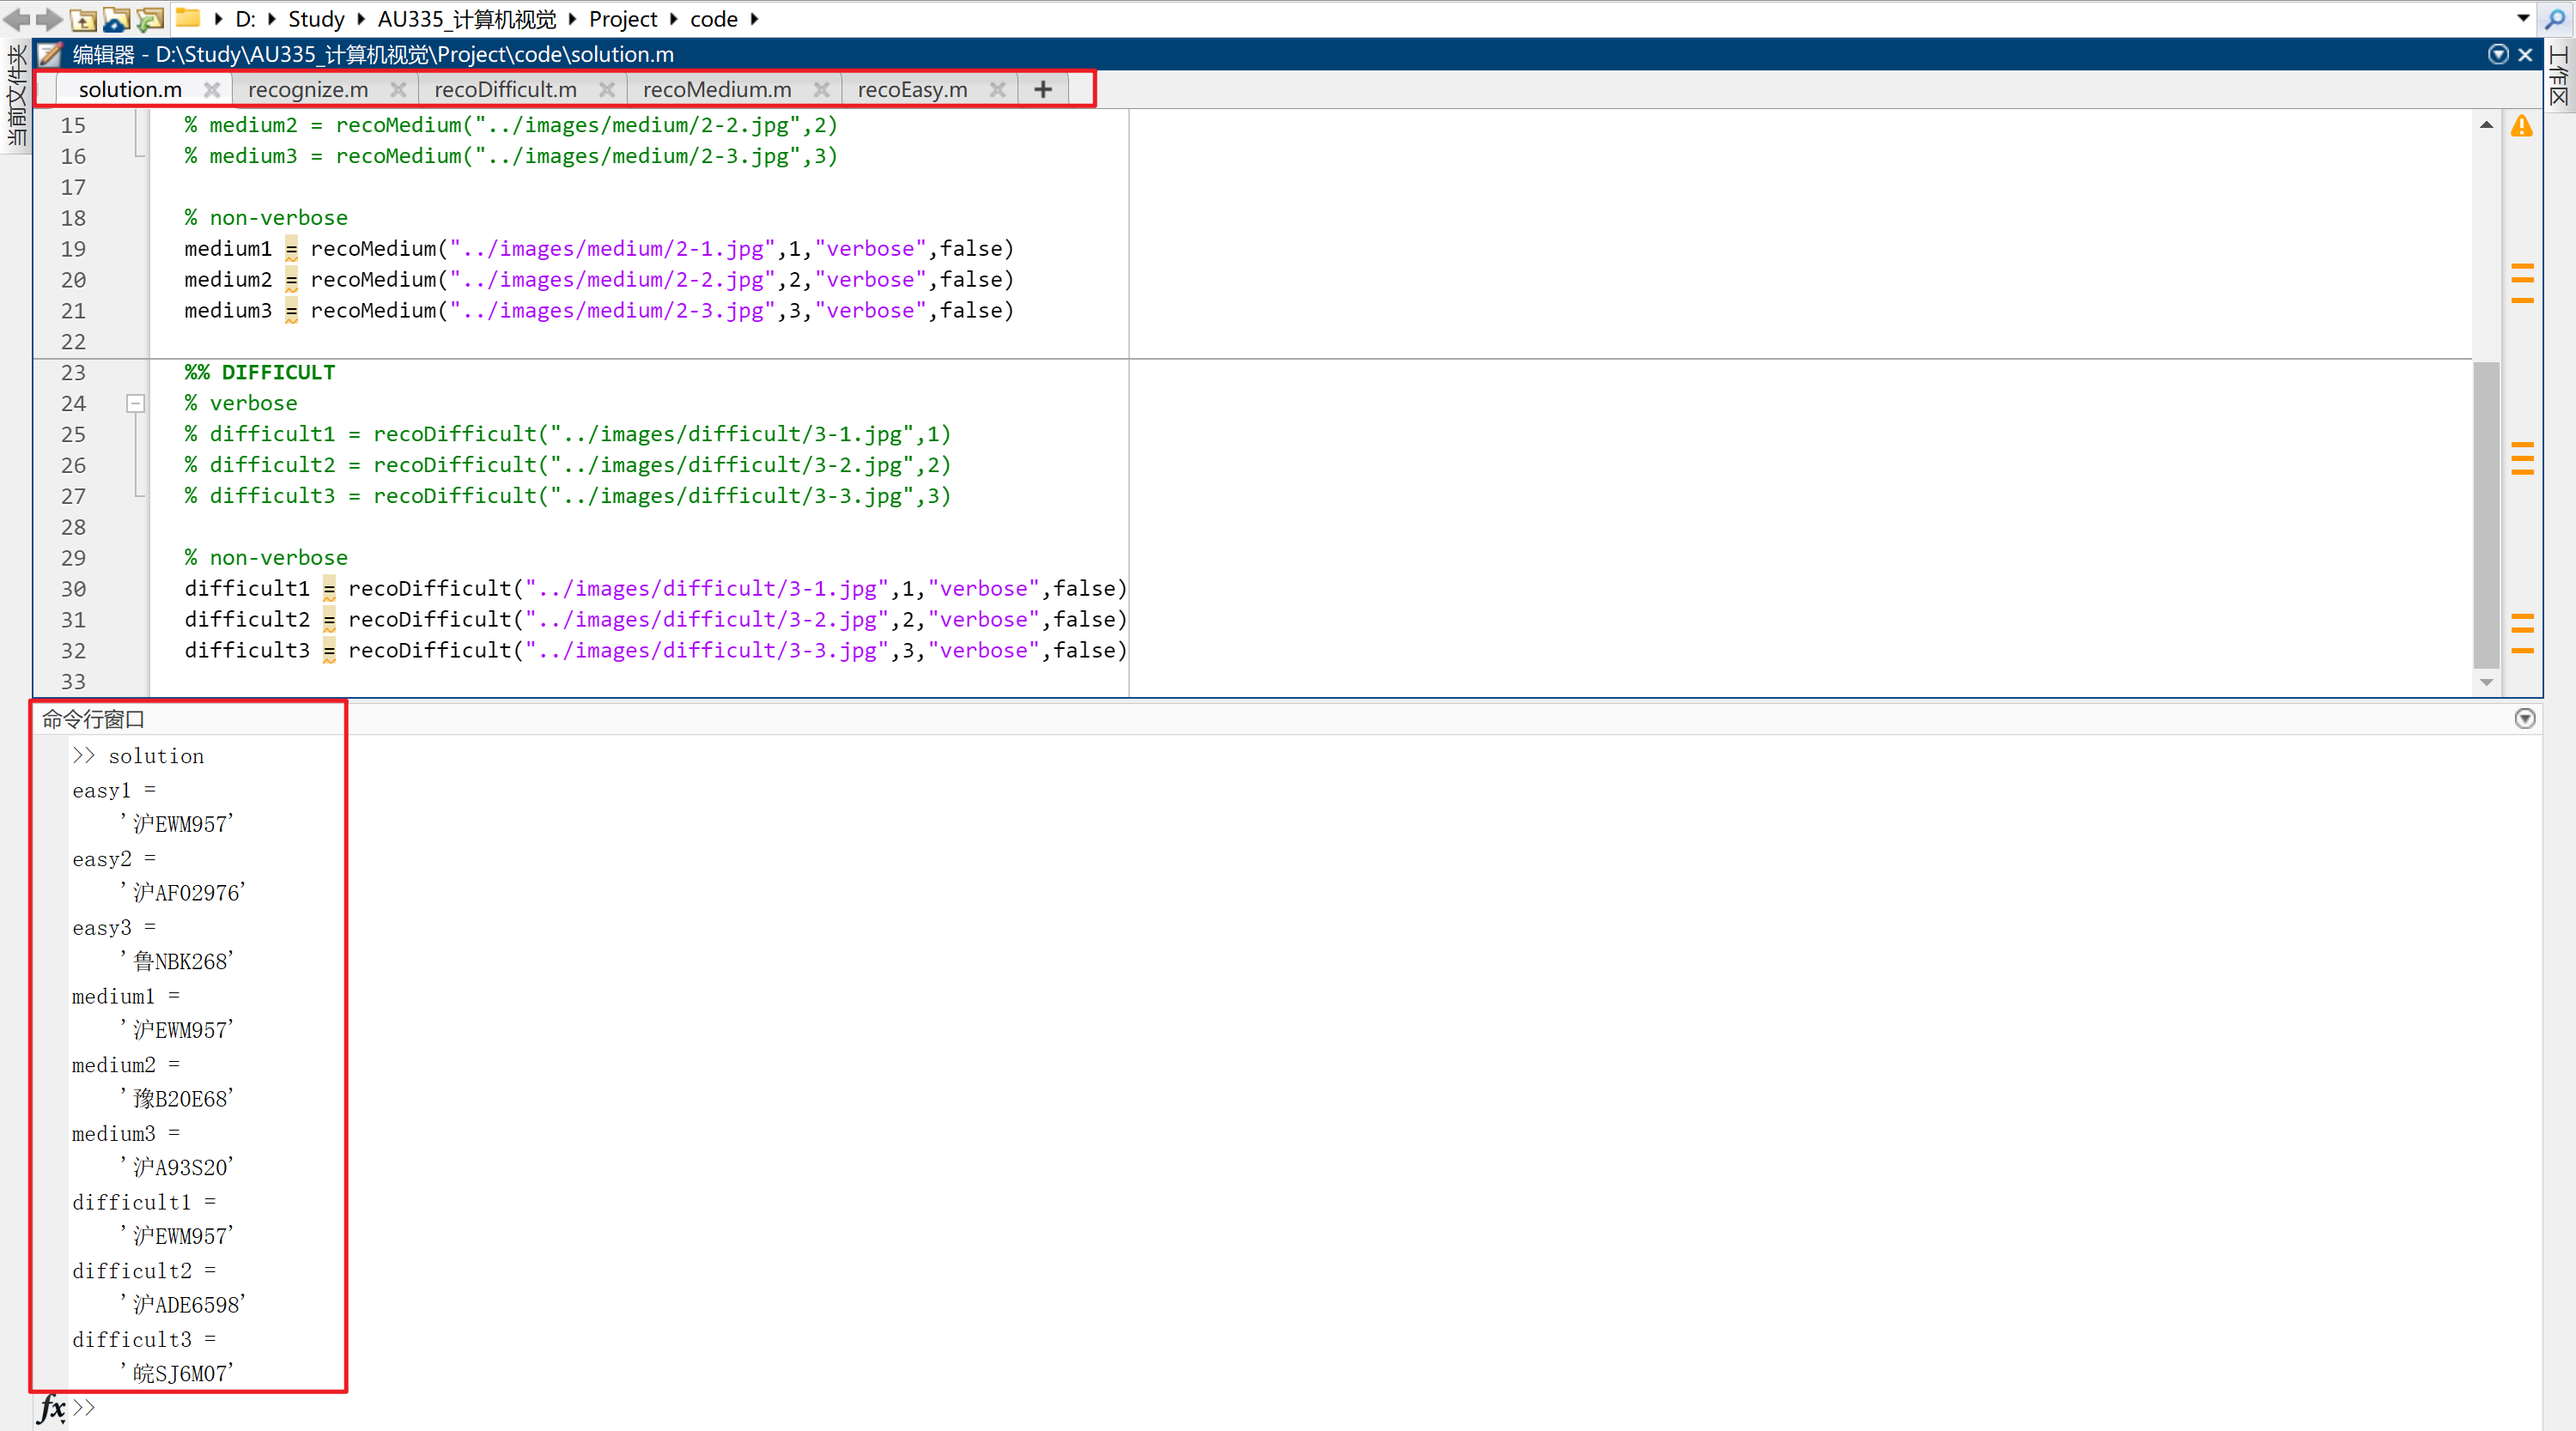
\includegraphics[width=.9\textwidth]{./img/res.png}
        \caption{results in cmd}
    \end{figure}

    \centering{\textbf{easy level}}

    \begin{minipage}{0.44\linewidth}
        \begin{figure}[H]
            \center
            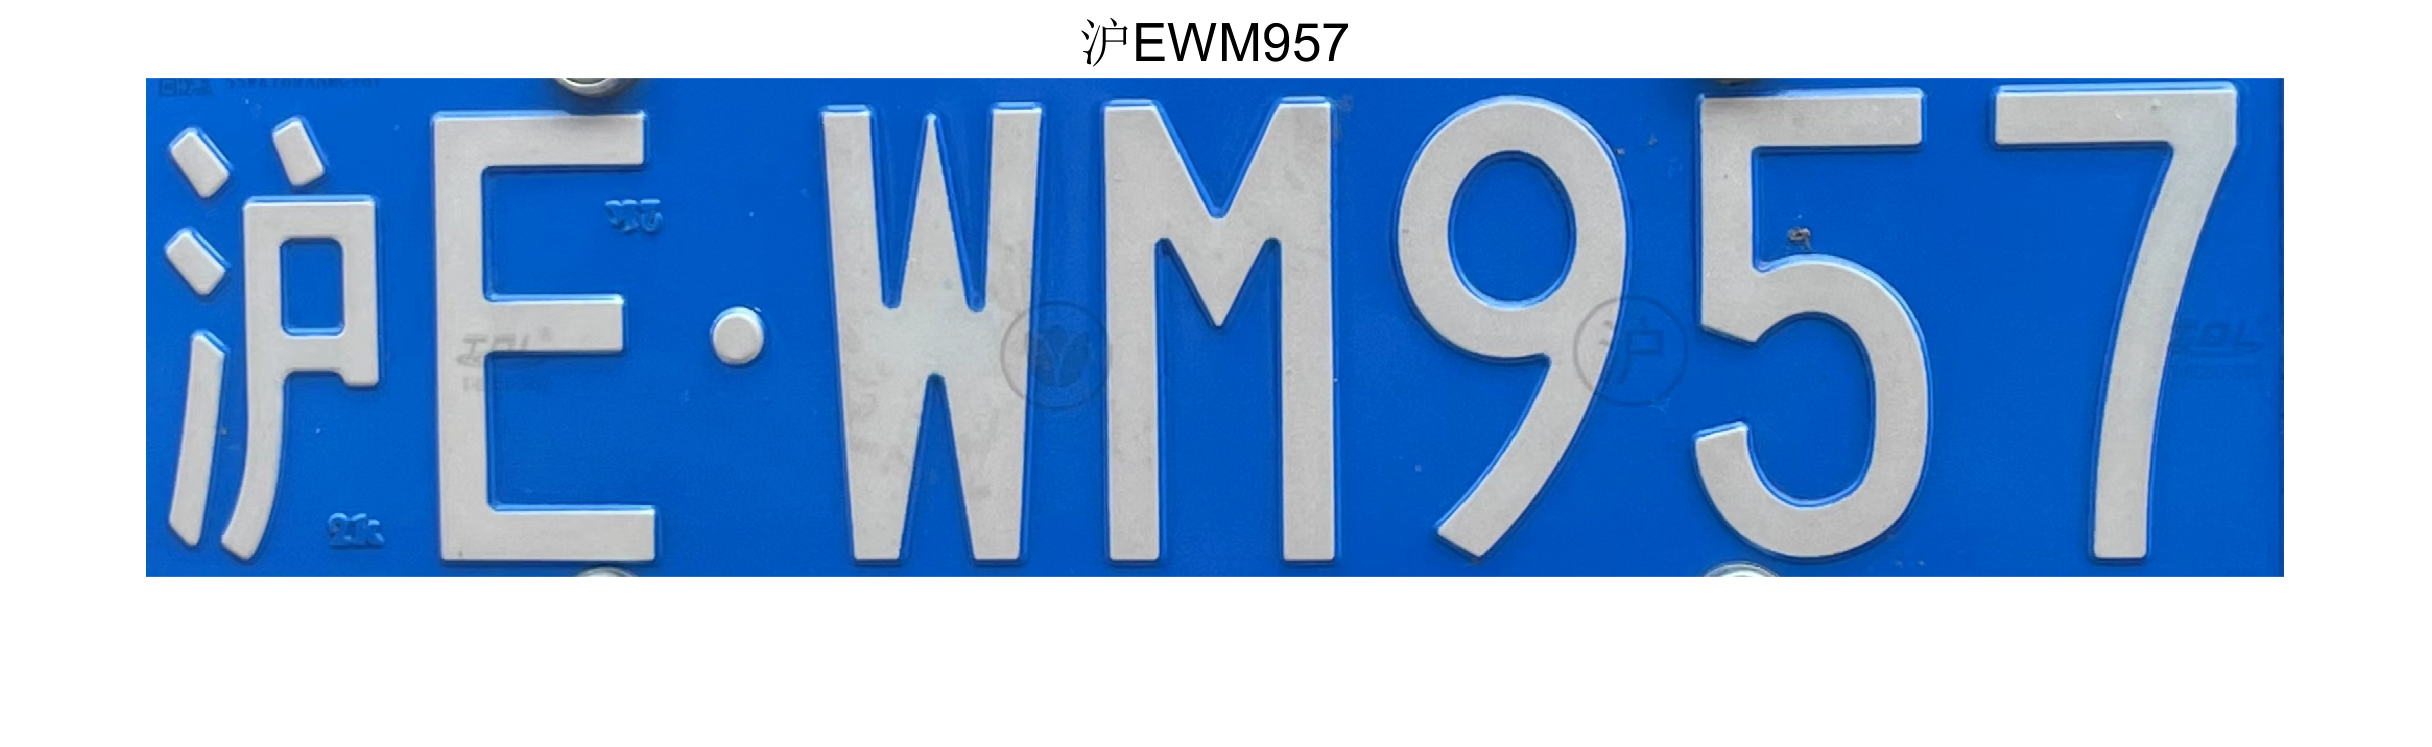
\includegraphics[width=\linewidth]{../result/easy/1-1.png}
            \caption{1-1.jpg: 沪EWM957}
        \end{figure}
    \end{minipage}
    \hfill
    \begin{minipage}{0.44\linewidth}
        \begin{figure}[H]
            \center
            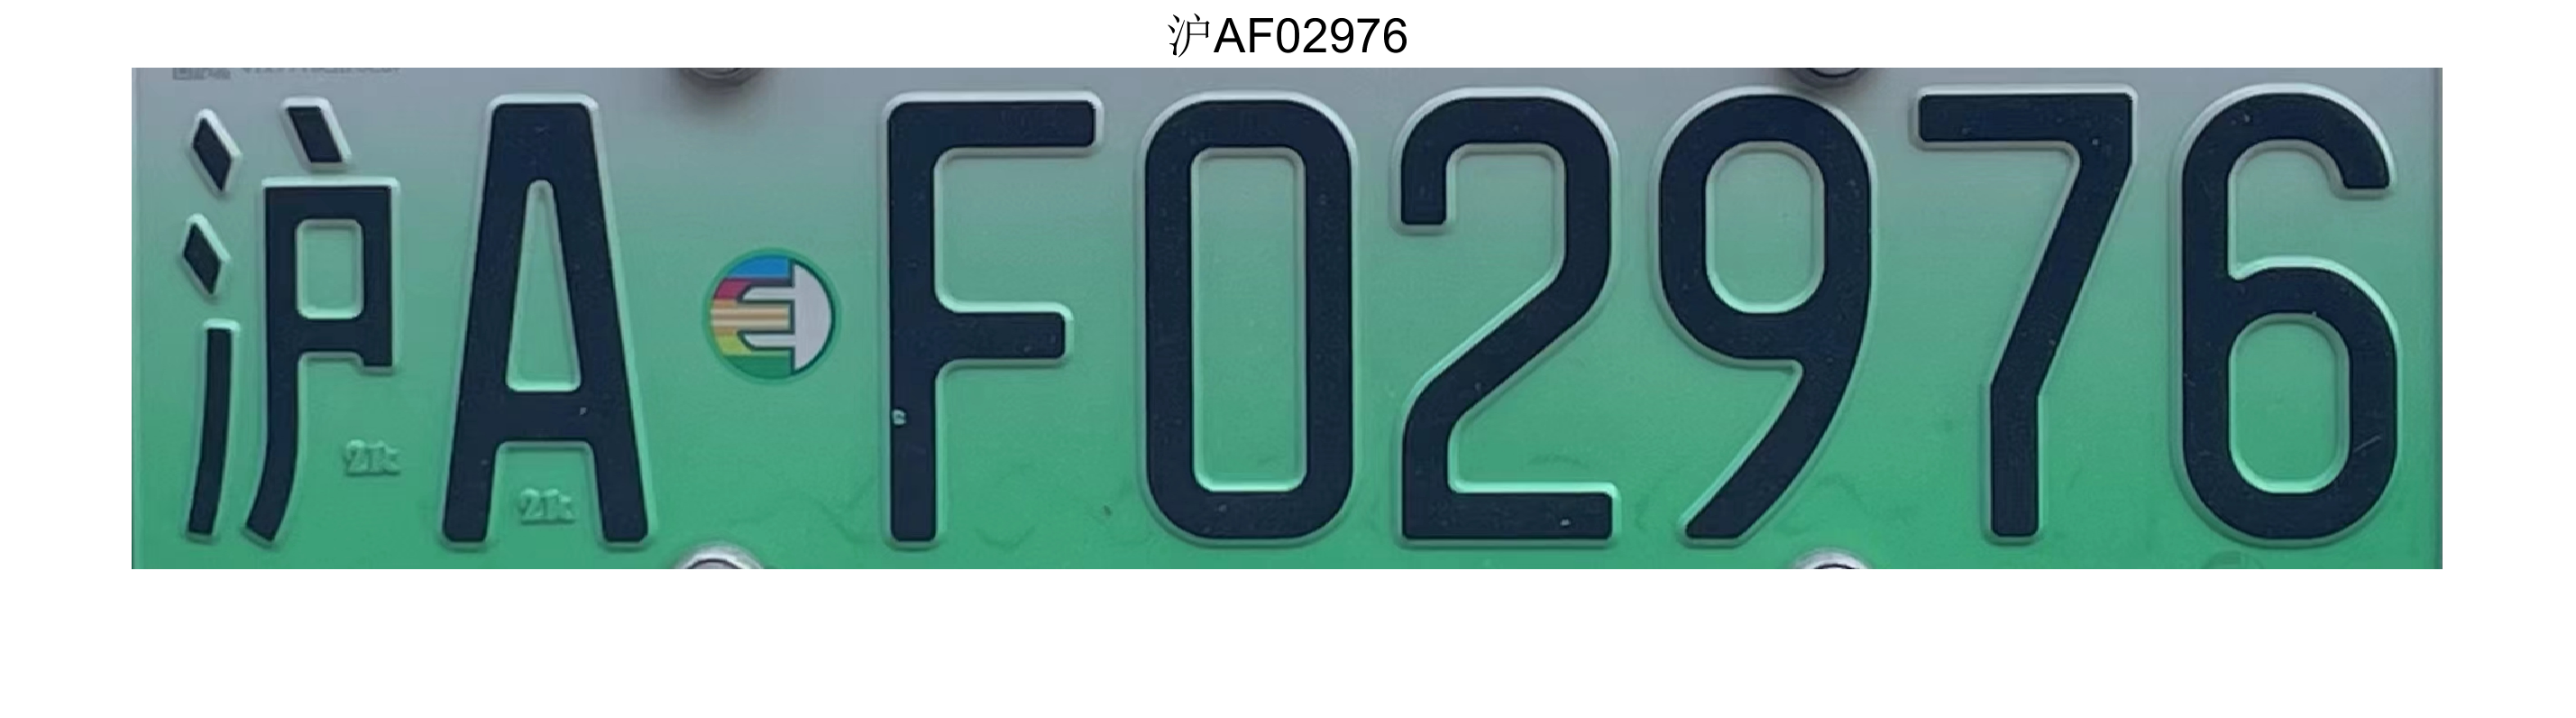
\includegraphics[width=\linewidth]{../result/easy/1-2.png}
            \caption{1-2.jpg: 沪AF02976}
        \end{figure}
    \end{minipage}
    \par
    \begin{minipage}{0.44\linewidth}
        \begin{figure}[H]
            \center
            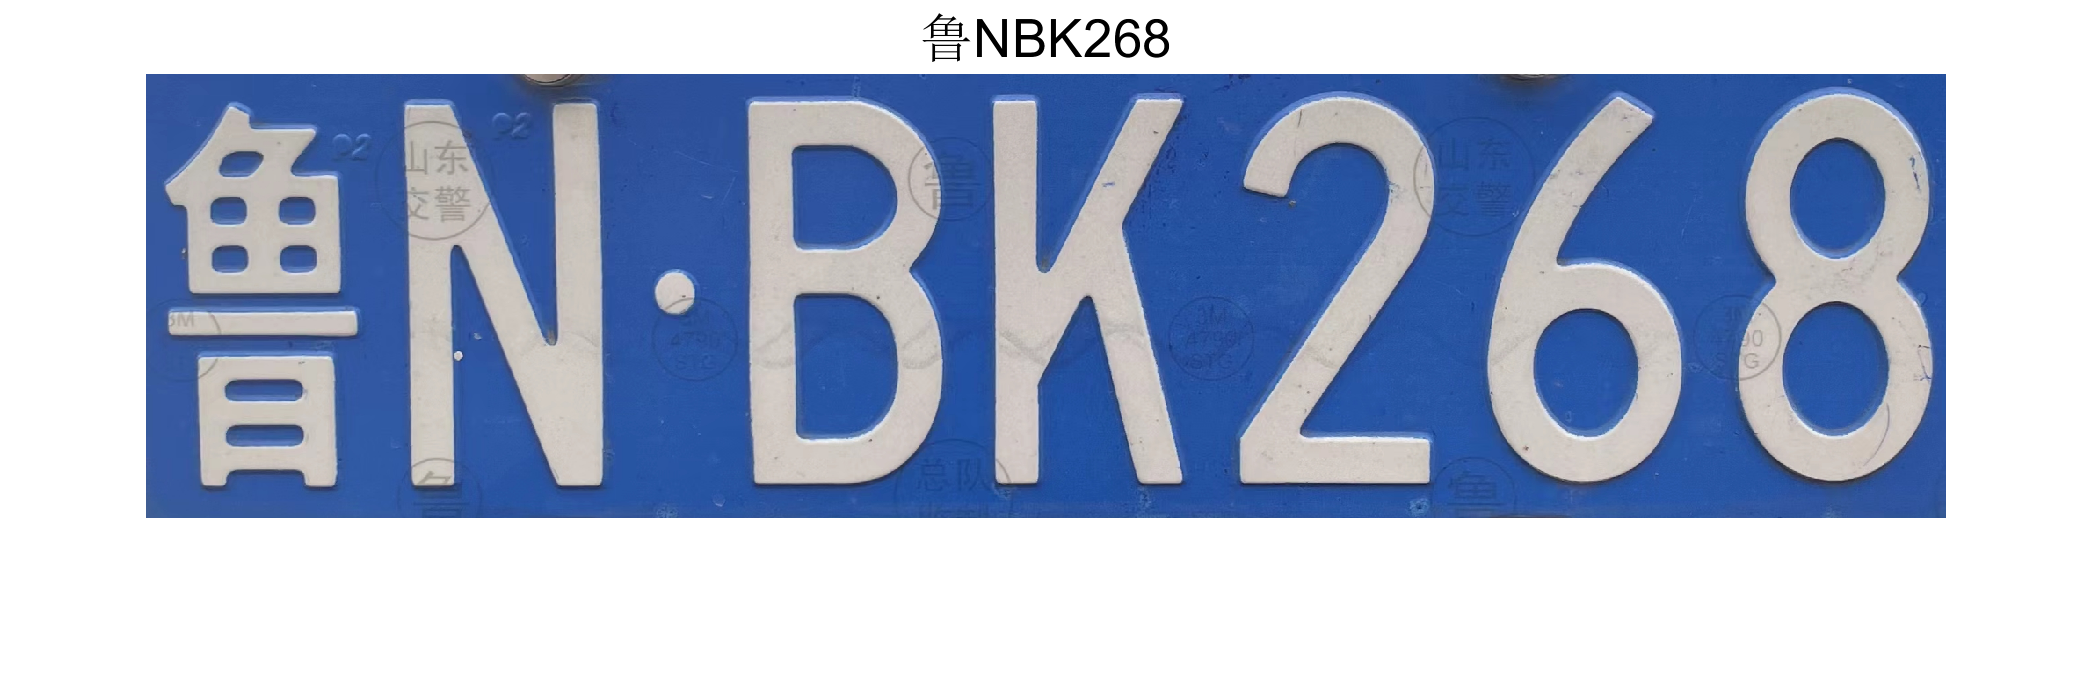
\includegraphics[width=\linewidth]{../result/easy/1-3.png}
            \caption{1-3.jpg: 鲁NBK268} 
        \end{figure}
    \end{minipage}
    \hfill
    \begin{minipage}{0.44\linewidth}
        
    \end{minipage}
    \par

    \centering{\textbf{medium level}}

    \begin{minipage}{0.44\linewidth}
        \begin{figure}[H]
            \center
            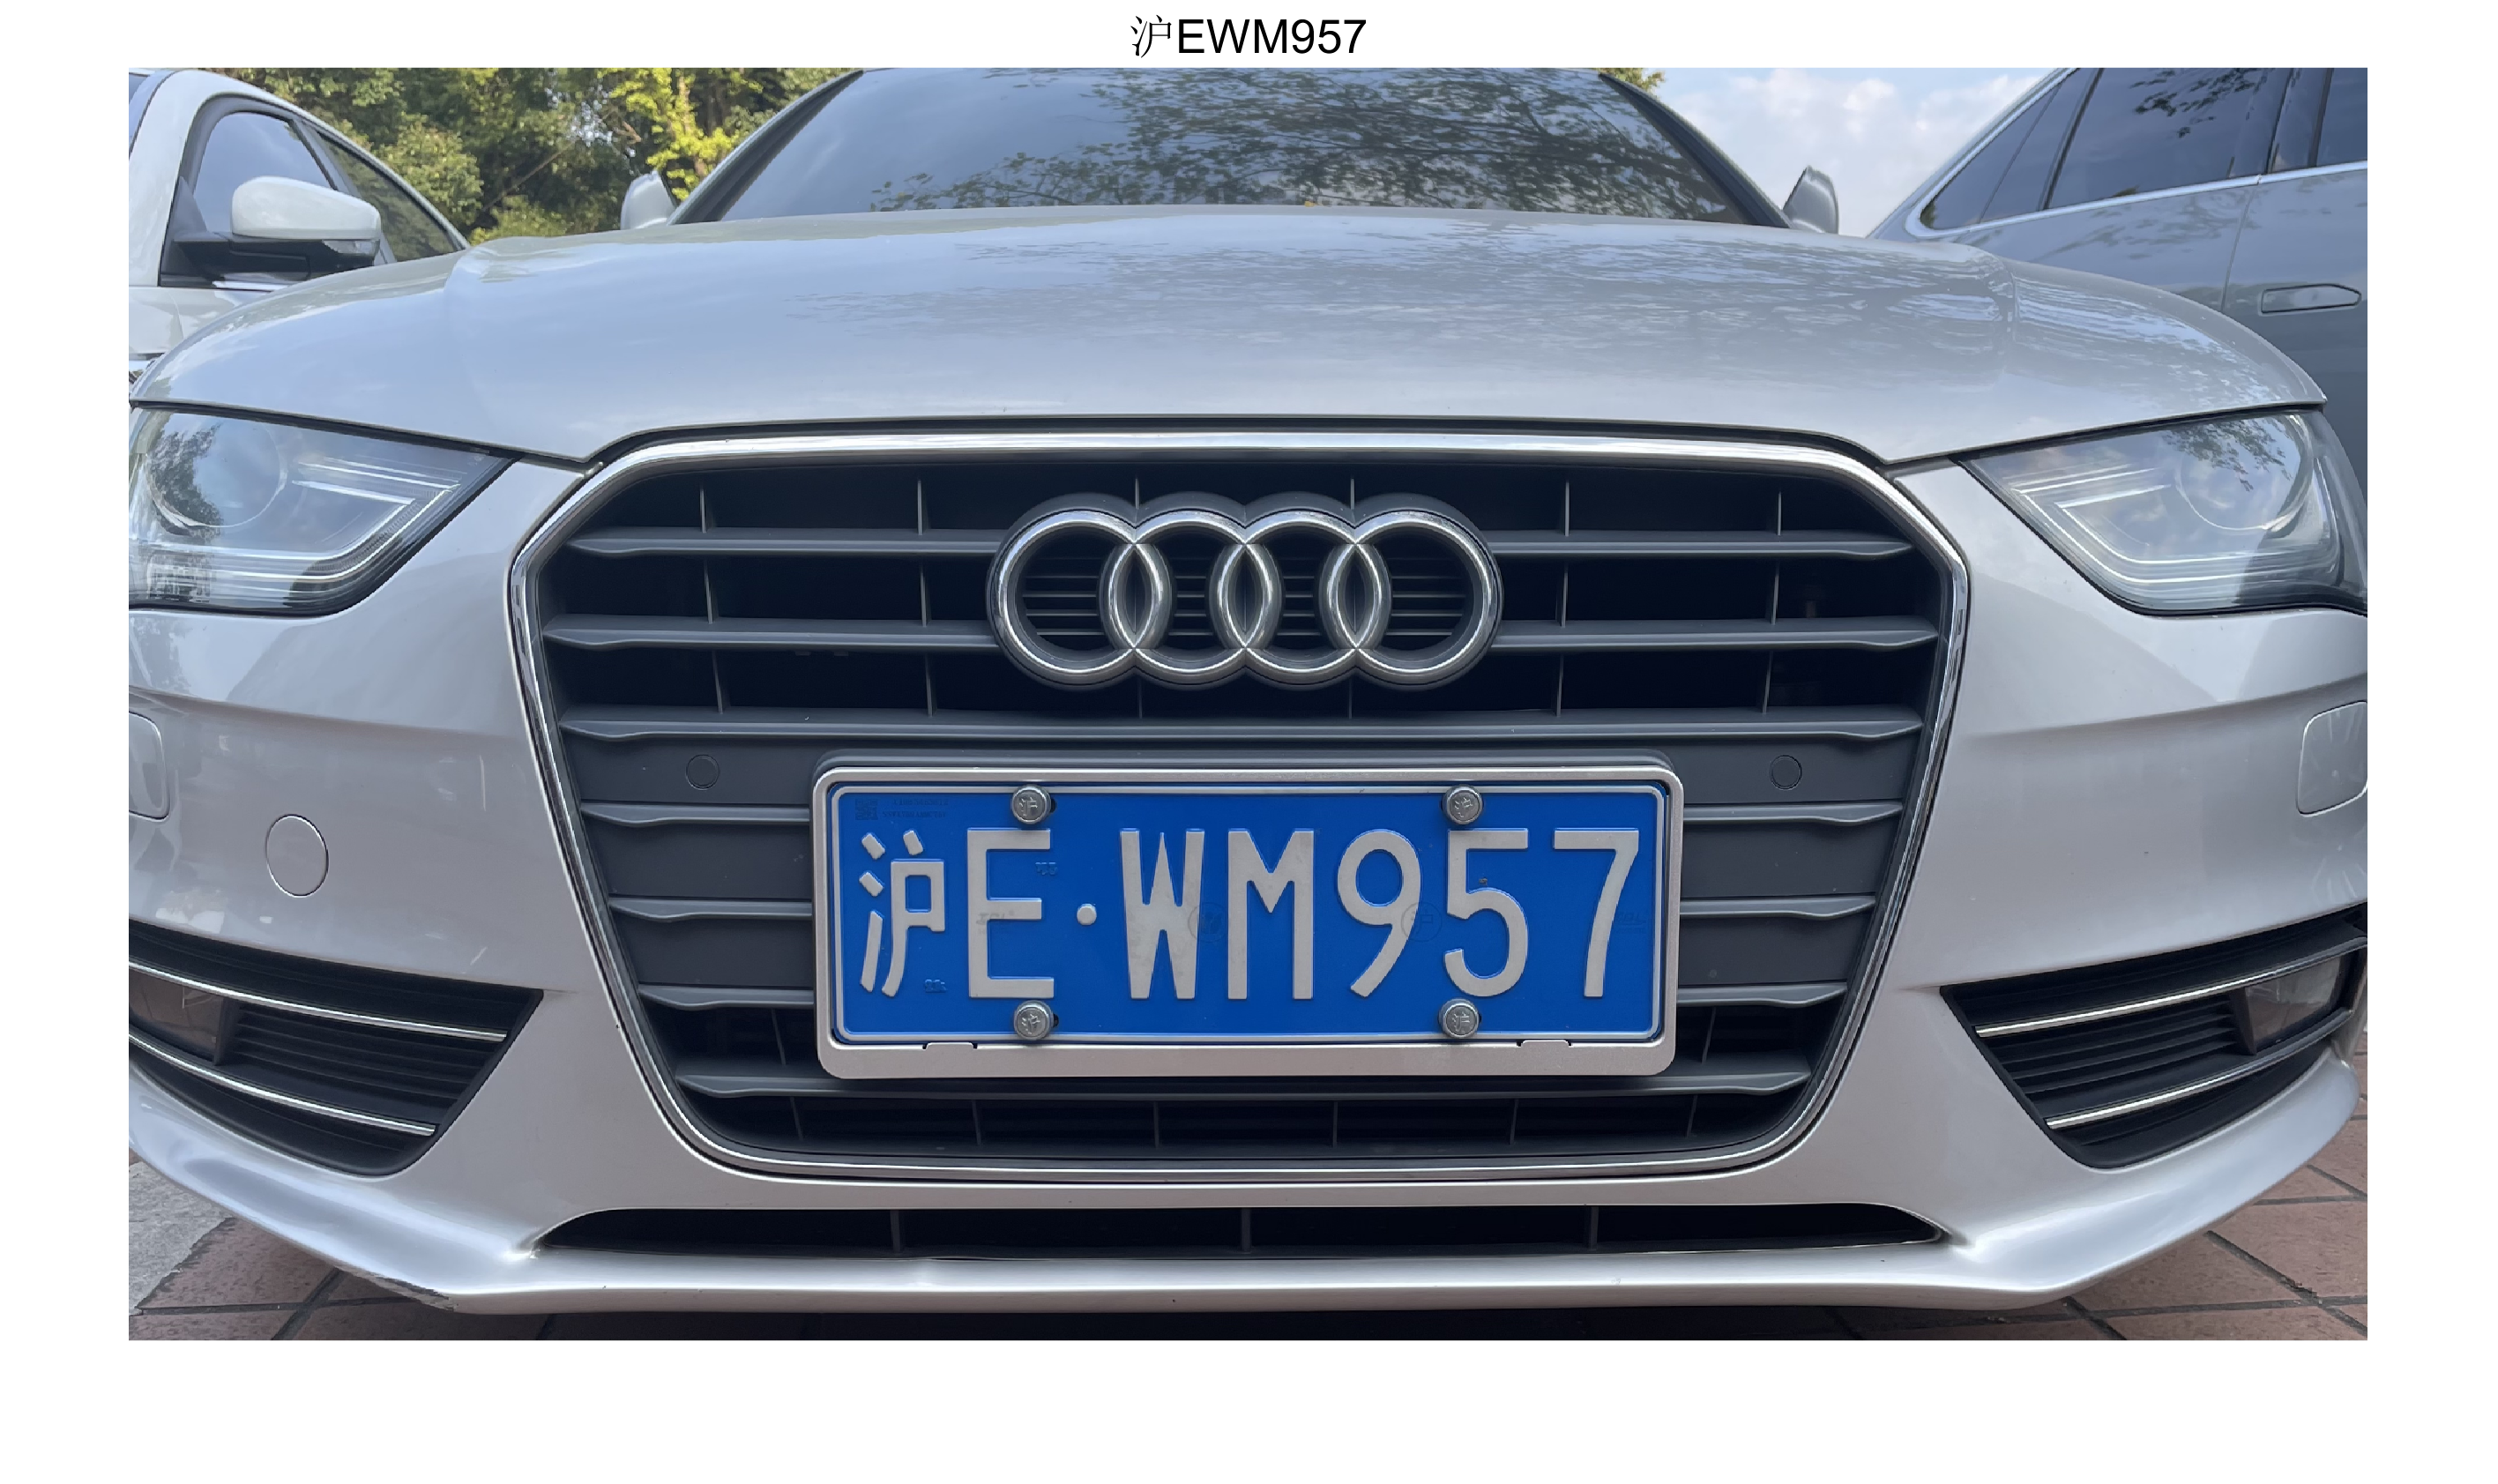
\includegraphics[width=\linewidth]{../result/medium/2-1.png}
            \caption{2-1.jpg: 沪EWM957}
        \end{figure}
    \end{minipage}
    \hfill
    \begin{minipage}{0.44\linewidth}
        \begin{figure}[H]
            \center
            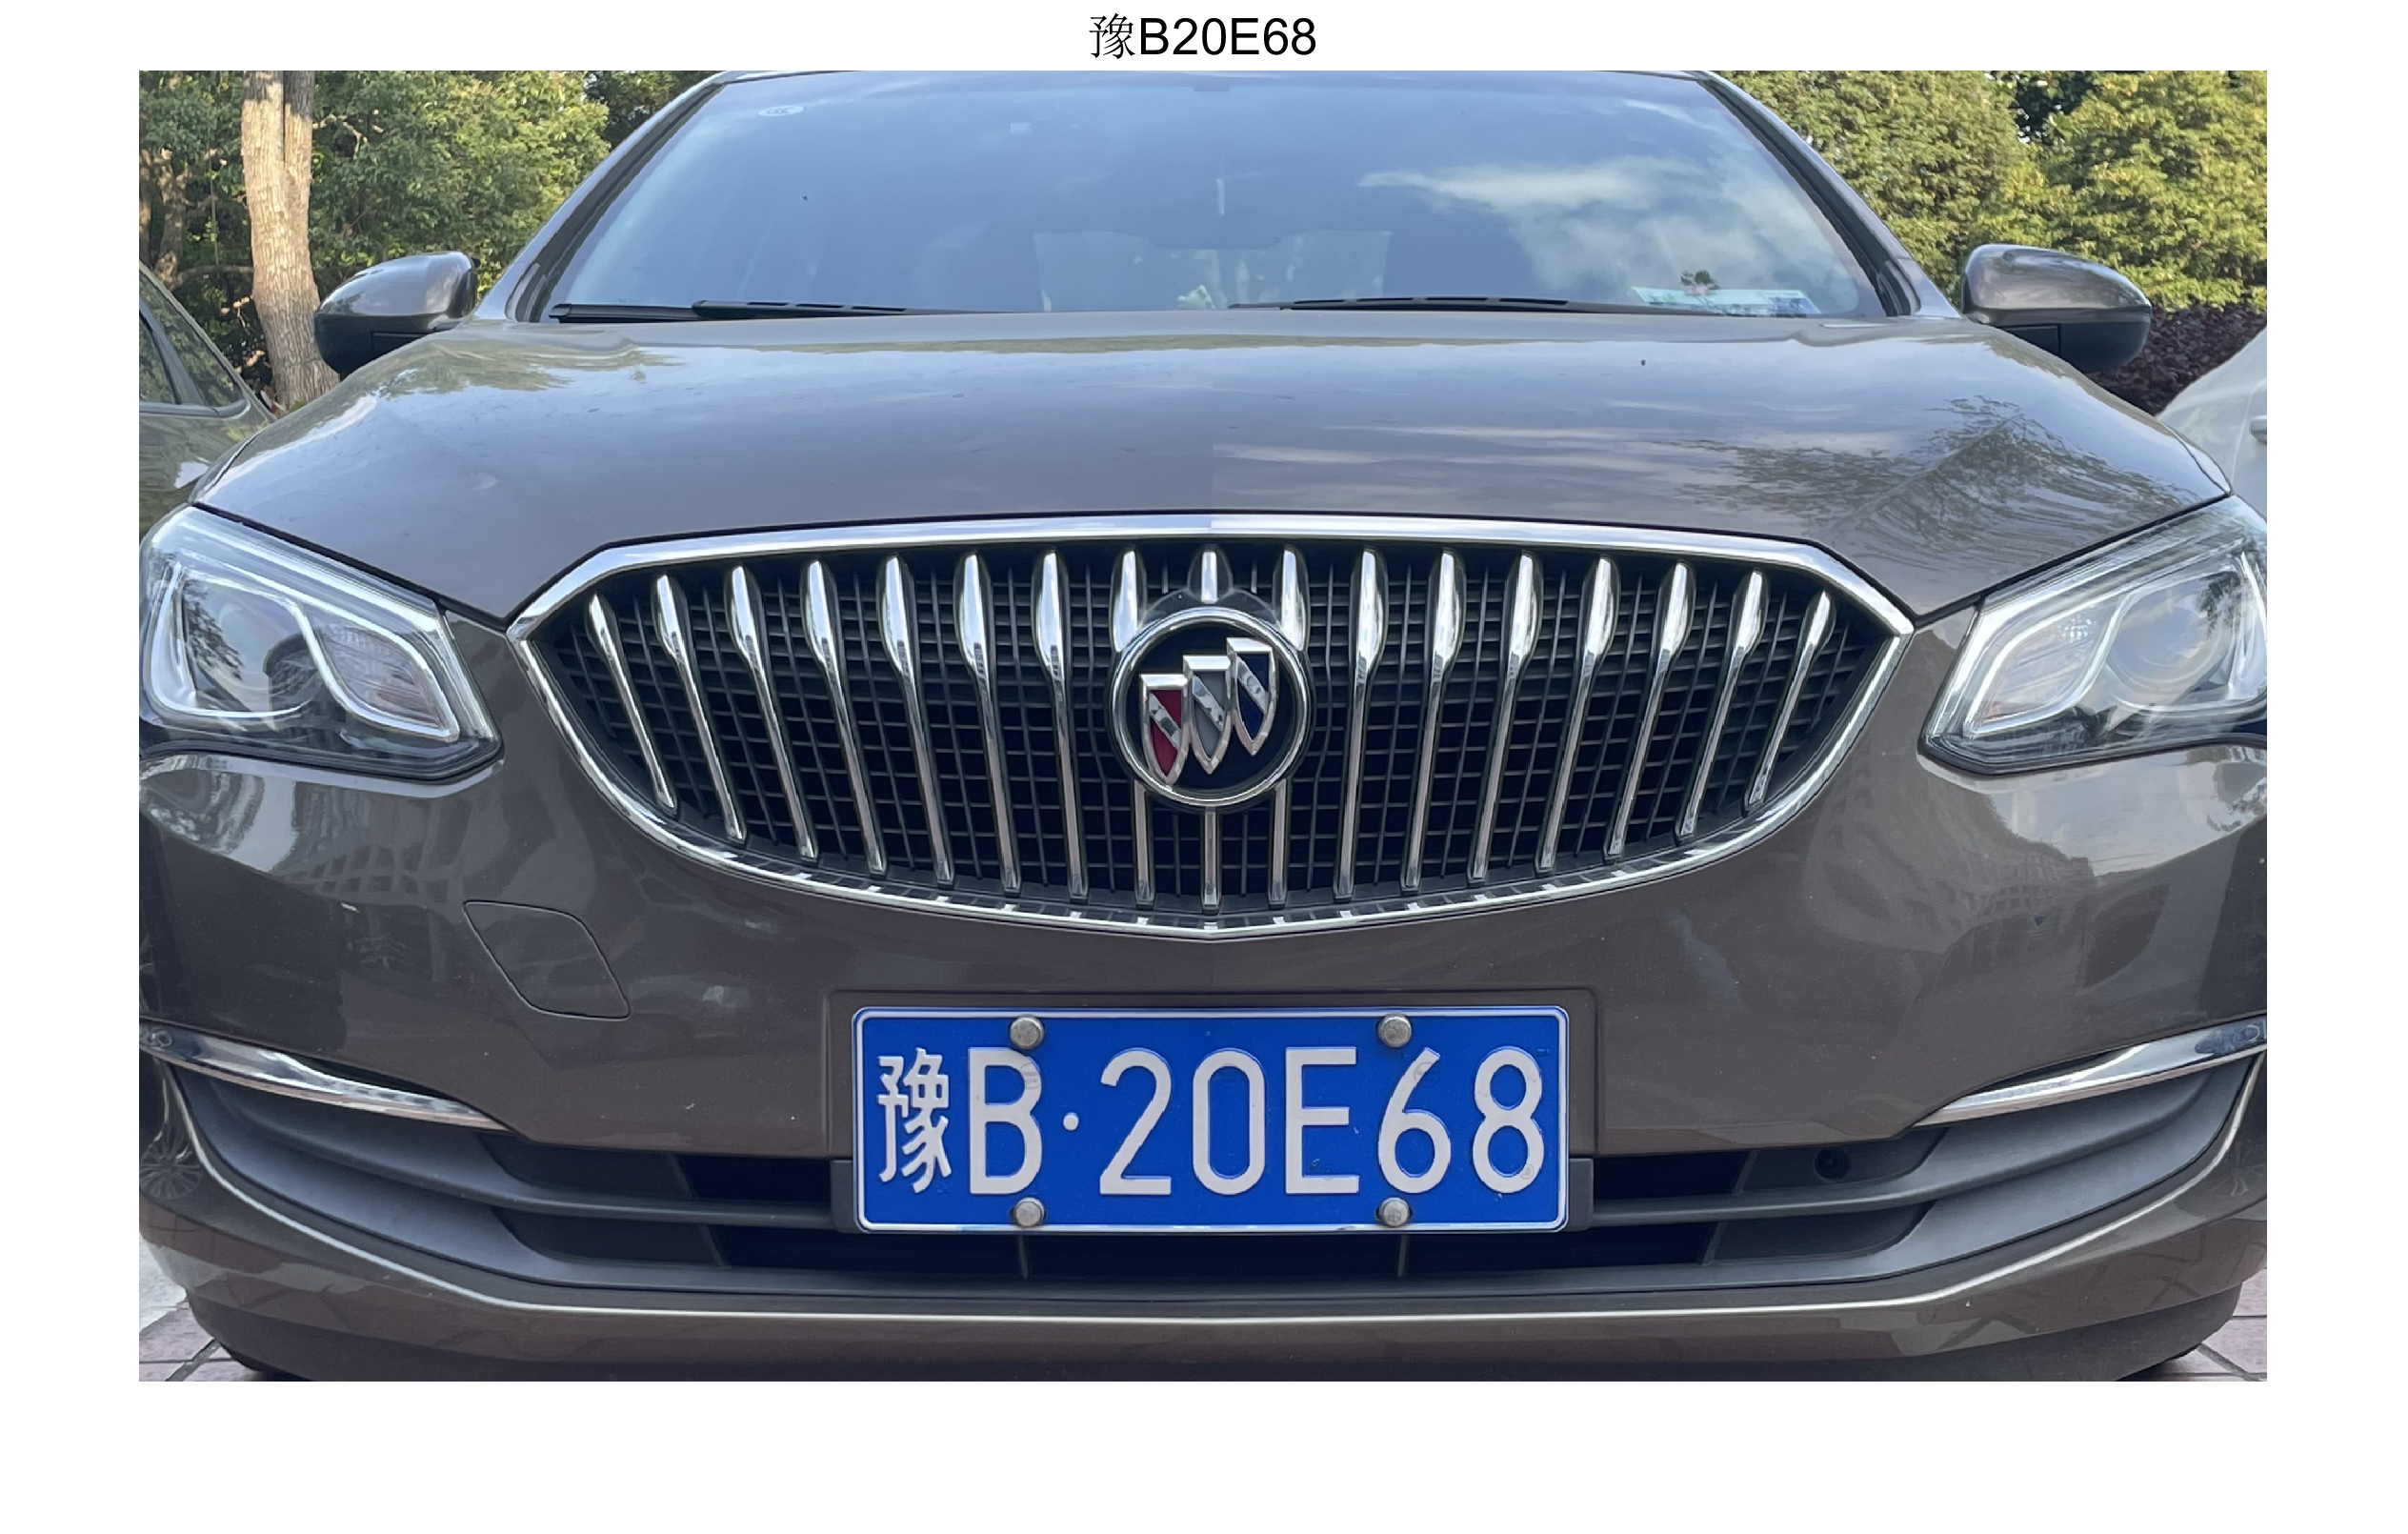
\includegraphics[width=\linewidth]{../result/medium/2-2.png}
            \caption{2-2.jpg: 豫B20E68}
        \end{figure}
    \end{minipage}
    \par
    \begin{minipage}{0.44\linewidth}
        \begin{figure}[H]
            \center
            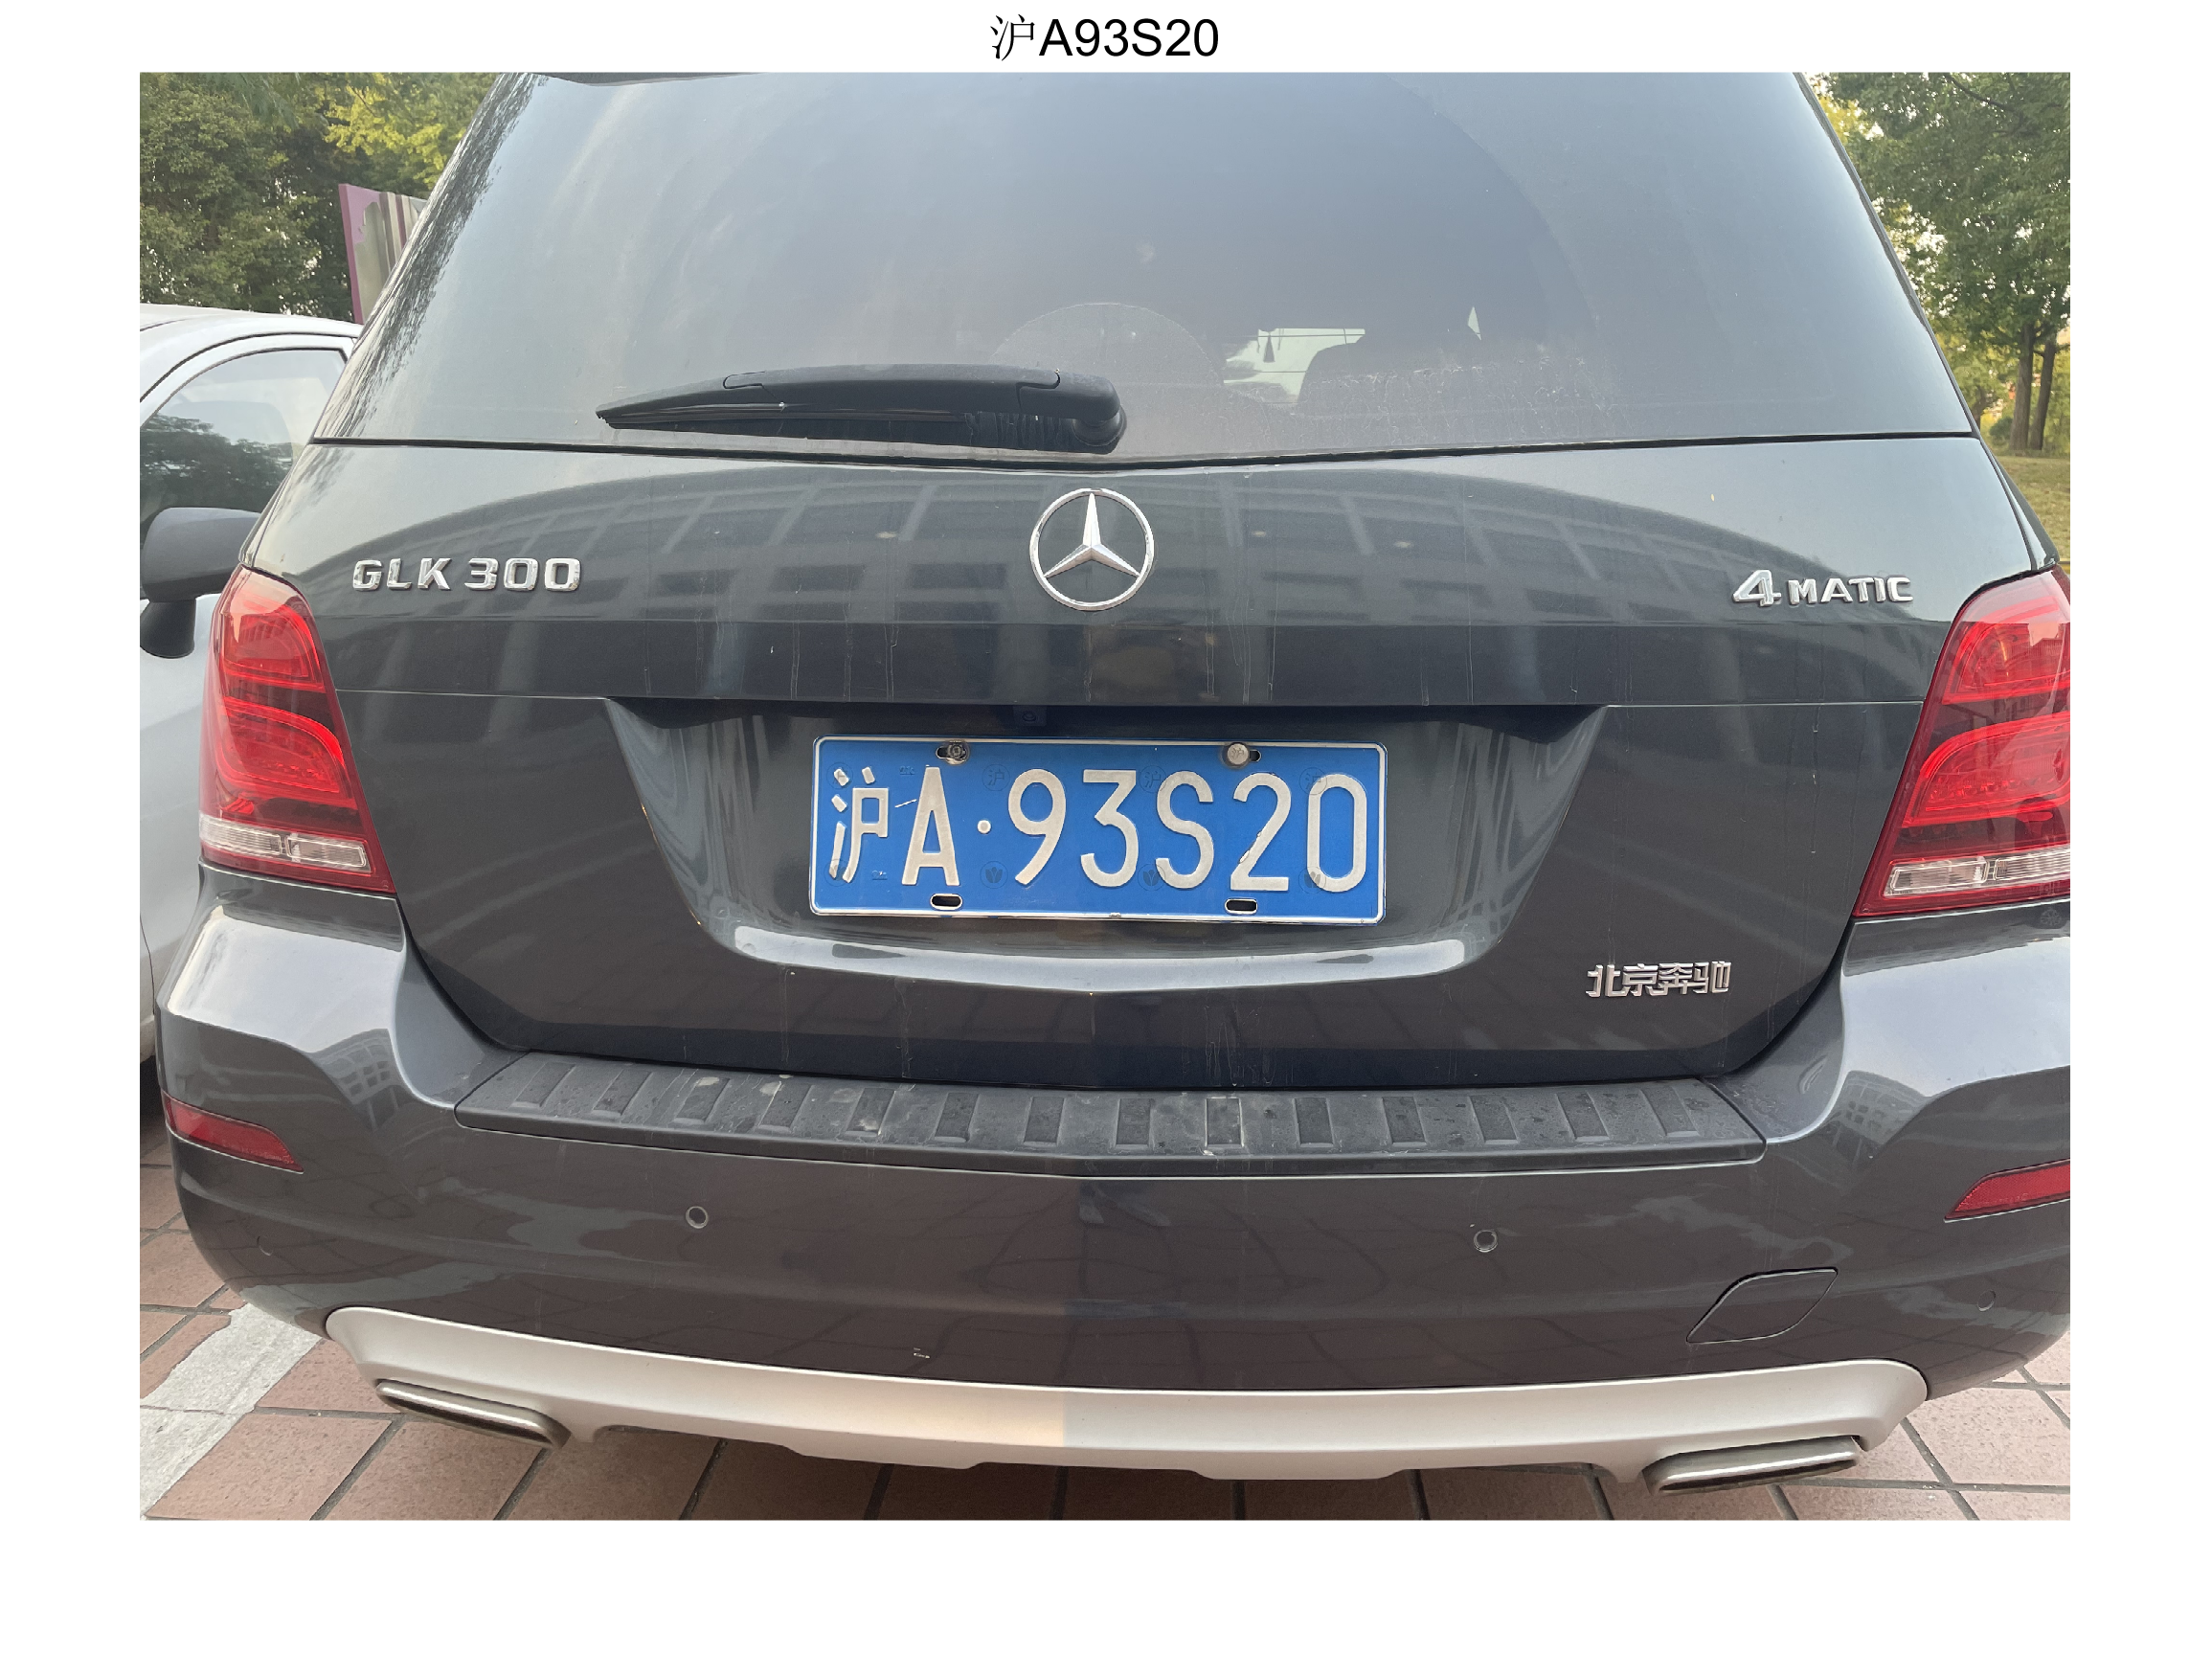
\includegraphics[width=\linewidth]{../result/medium/2-3.png}
            \caption{2-3.jpg: 沪A93S20} 
        \end{figure}
    \end{minipage}
    \hfill
    \begin{minipage}{0.44\linewidth}
        
    \end{minipage}
    \par

    \centering{\textbf{difficult level}}

    \begin{minipage}{0.44\linewidth}
        \begin{figure}[H]
            \center
            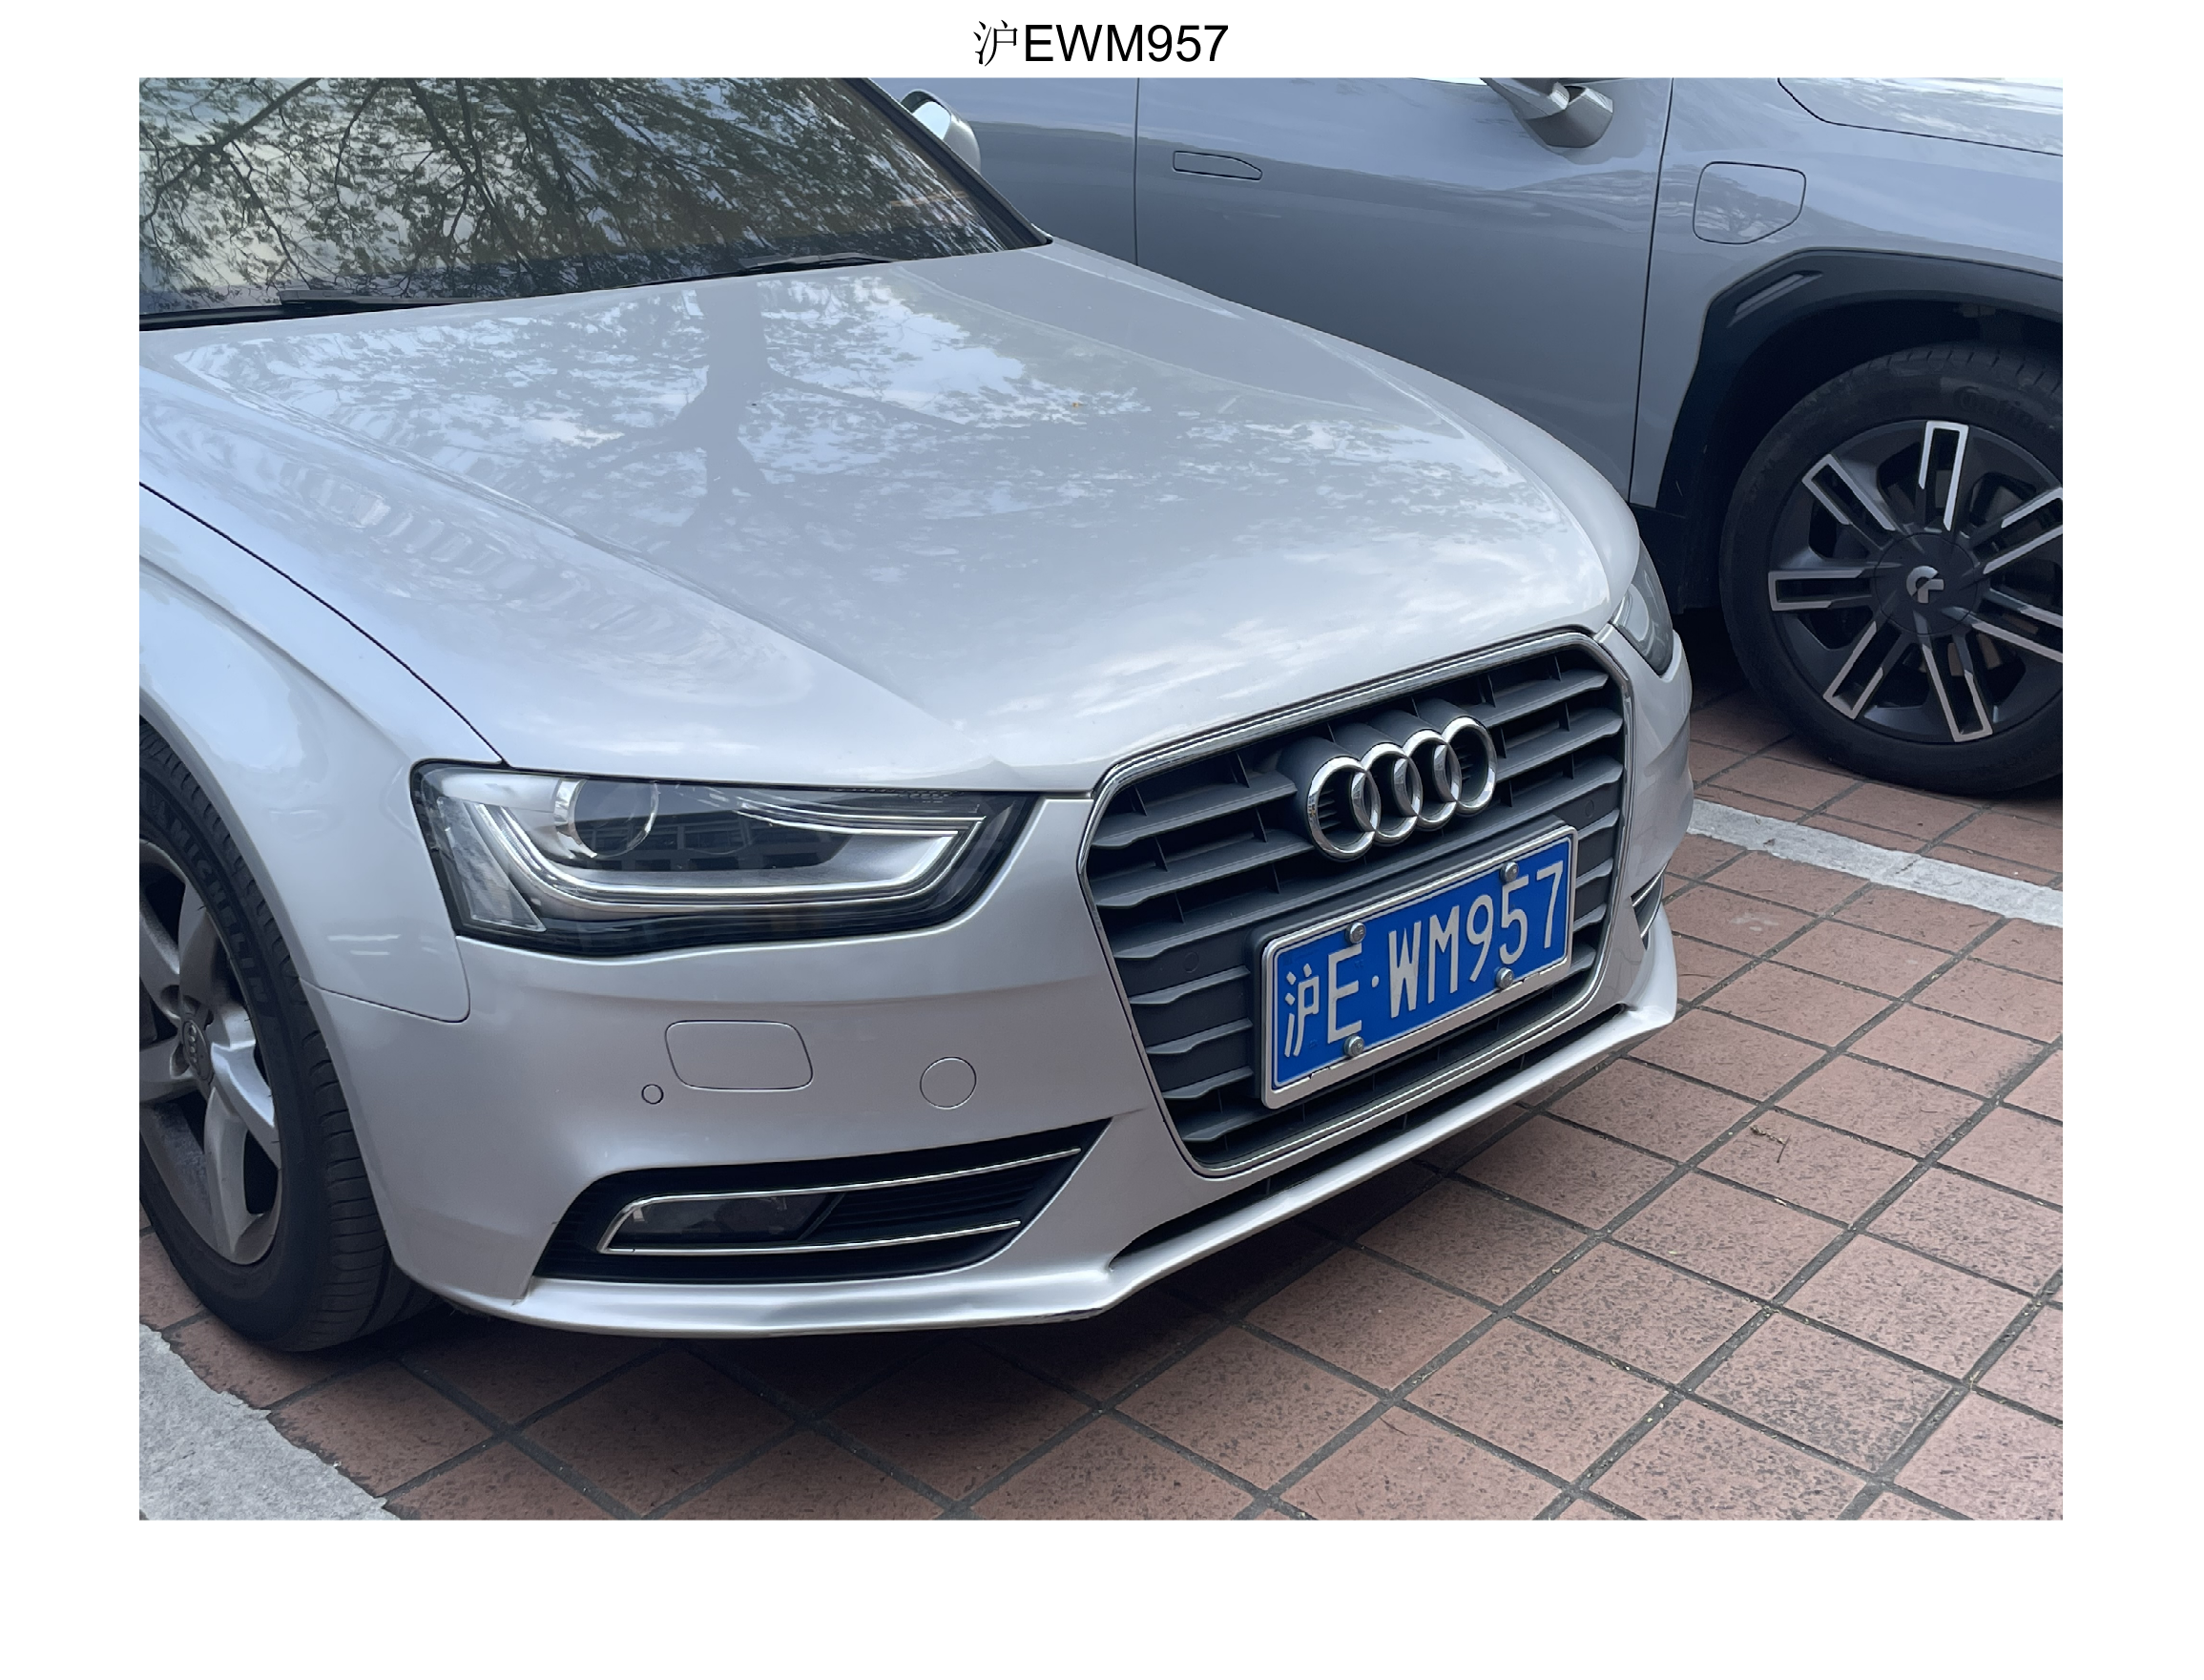
\includegraphics[width=\linewidth]{../result/difficult/3-1.png}
            \caption{3-1.jpg: 沪EWM957}
        \end{figure}
    \end{minipage}
    \hfill
    \begin{minipage}{0.44\linewidth}
        \begin{figure}[H]
            \center
            \includegraphics[width=\linewidth]{../result/difficult/3-2.png}
            \caption{3-2.jpg: 沪ADE6598}
        \end{figure}
    \end{minipage}
    \par
    \begin{minipage}{0.44\linewidth}
        \begin{figure}[H]
            \center
            \includegraphics[width=\linewidth]{../result/difficult/3-3.png}
            \caption{3-3.jpg: 皖SJ6M07} 
        \end{figure}
    \end{minipage}
    \hfill
    \begin{minipage}{0.44\linewidth}
        
    \end{minipage}
    \par

    \section{支撑文件结构说明}
    \begin{itemize}
        \item code文件夹下是所有的程序文件。
              \begin{itemize}
                  \item solution.m为顶层逻辑代码,可以直接运行该文件获取识别结果。
                  \item recognize.m为封装的实现字符分割与识别算法的函数。
                  \item recoEasy.m, recoMedium.m, recoDifficult.m分别为识别三类难度级别图像的封装函数。
                  \item ``verbose''为这些函数的可选参数,以控制是否详细显示识别过程的信息,默认值为``true''。
                  \item ``whiteCountPerColumnThreshold''为这些函数的可选参数,为白色像素点分割阈值,默认值为``5''。
                  \item 部分程序思路以注释的形式在代码中给出。
              \end{itemize}
        \item article文件夹下是本篇论文的\LaTeX 源文件及文中的所有插图。
        \item result文件夹下是车牌识别的结果,结果以图片标题的形式在图中标出。
    \end{itemize}


    % \section{字符分割识别代码}
    % \lstinputlisting[language=Matlab]{../code/recognize.m}

\end{appendices}

\end{document}